%% Commands for TeXCount
%TC:macro \cite [option:text,text]
%TC:macro \citep [option:text,text]
%TC:macro \citet [option:text,text]
%TC:envir table 0 1
%TC:envir table* 0 1
%TC:envir tabular [ignore] word
%TC:envir displaymath 0 word
%TC:envir math 0 word
%TC:envir comment 0 0

\documentclass[acmsmall]{acmart}

%% ------ Packages & Setup Starts ------
\usepackage[utf8]{inputenc}
\usepackage[T1]{fontenc}
\usepackage{graphicx}
\usepackage{hyperref}
\usepackage{url}
\usepackage{tabularx}
\usepackage{booktabs}
\usepackage{longtable}
\usepackage{pdflscape}
\usepackage{tikz}
\usepackage{pgfplots}
\usepackage{pgf-pie}
\usepackage{pgfplotstable}
\usepackage{colortbl}
\usepackage{xcolor}
\usepackage[most]{tcolorbox}
\usepackage[capitalize, nameinlink, noabbrev]{cleveref}
\usepackage{textalpha}
\usepackage{rotating}
\usepackage{algorithm}
\usepackage{subcaption}
\usepackage{multirow}
\usepackage{array}

\tcbuselibrary{breakable}

% Define the theme box style
\usetikzlibrary{calc, shapes.geometric, arrows, positioning, fit}

\newcounter{themecounter}
\setcounter{themecounter}{0}

\newtcolorbox{themebox}[1]{
  enhanced,
  breakable,
  colback=white,
  colframe=blue!70!black,
  colbacktitle=white,
  coltitle=blue!70!black,
  title={\textbf{\normalsize Theme \stepcounter{themecounter}\arabic{themecounter}: #1}},
  fonttitle=\bfseries,
  halign title=left,
  boxrule=1pt,
  sharp corners,
  toptitle=10pt,
  bottomtitle=10pt,
  lefttitle=12pt,
  righttitle=12pt
}

\newtcolorbox{algorithmbox}[1]{
  enhanced,
  breakable,
  colback=white,
  colframe=black!50,
  colbacktitle=black!10,
  coltitle=black,
  title={\textbf{\normalsize #1}},
  fonttitle=\bfseries,
  halign title=left,
  boxrule=0.5pt,
  sharp corners,
  toptitle=8pt,
  bottomtitle=8pt,
  lefttitle=10pt,
  righttitle=10pt,
  left=8pt,
  right=8pt,
  top=8pt,
  bottom=8pt
}

\pgfplotsset{compat=newest}

\newcommand{\ATM}[1]{\textcolor{red}{#1}}

\renewcommand{\tabularxcolumn}[1]{>{\arraybackslash}m{#1}}

%% ------ Packages & Setup Ends ------

%% ----- Front Matters Starts -----

%% Rights management information.  This information is sent to you
%% when you complete the rights form.  These commands have SAMPLE
%% values in them; it is your responsibility as an author to replace
%% the commands and values with those provided to you when you
%% complete the rights form.
\setcopyright{acmlicensed}
\copyrightyear{2025}
\acmYear{2025}
\acmDOI{XXXXXXX.XXXXXXX}

%% These commands are for a JOURNAL article.
\acmJournal{JACM}
\acmVolume{00}
\acmNumber{0}
\acmArticle{000}
\acmMonth{13}

%% Submission ID.
%% Use this when submitting an article to a sponsored event. You'll
%% receive a unique submission ID from the organizers
%% of the event, and this ID should be used as the parameter to this command.
%%\acmSubmissionID{123-A56-BU3}

%% ----- Front Matters Ends -----

\begin{document}

%% ----- Title Page Setup Starts -----

%% The "title" command has an optional parameter,
%% allowing the author to define a "short title" to be used in page headers.
\title{Numerical Methods and Distributed Computing for Deep Learning on Big Data}

%%
%% The "author" command and its associated commands are used to define
%% the authors and their affiliations.
%% Of note is the shared affiliation of the first two authors, and the
%% "authornote" and "authornotemark" commands
%% used to denote shared contribution to the research.
\author{Ben Trovato}
\authornote{Both authors are people.}
\email{trovato@corporation.com}
\orcid{1234-5678-9012}
\author{G.K.M. Tobin}
\authornotemark[1]
\email{webmaster@marysville-ohio.com}
\affiliation{%
    \institution{Institute for Clarity in Documentation}
    \city{Dublin}
    \state{Ohio}
    \country{USA}
}

\author{Marcellin Atemkeng}
\affiliation{%
    \institution{Department of Mathematics, Rhodes University}
    \city{Makhanda}
    \country{South Africa}
}

\author{Nguembang Fadja Arnaud}
\affiliation{%
    \institution{Department of Engineering, University of Ferrara}
    \city{Ferrara}
    \country{Italy}
}

\author{Brian Welman}
\affiliation{%
    \institution{Department of Physics \& Electronics, Rhodes University}
    \city{Makhanda}
    \country{South Africa}
}

\author{Stones Dalitso Chindipha}
\affiliation{%
    \institution{Department of Computer Science, Rhodes University}
    \city{Makhanda}
    \country{South Africa}
}

%%
%% By default, the full list of authors will be used in the page
%% headers. Often, this list is too long, and will overlap
%% other information printed in the page headers. This command allows
%% the author to define a more concise list
%% of authors' names for this purpose.
\renewcommand{\shortauthors}{Trovato et al.}

%%
%% The abstract is a short summary of the work to be presented in the
%% article.
\begin{abstract}
    A clear and well-documented \LaTeX\ document is presented as an
    article formatted for publication by ACM in a conference proceedings
    or journal publication. Based on the ``acmart'' document class, this
    article presents and explains many of the common variations, as well
    as many of the formatting elements an author may use in the
    preparation of the documentation of their work.
\end{abstract}

%%
%% The code below is generated by the tool at http://dl.acm.org/ccs.cfm.
%% Please copy and paste the code instead of the example below.
%%
\begin{CCSXML}
    <ccs2012>
    <concept>
    <concept_id>00000000.0000000.0000000</concept_id>
    <concept_desc>Do Not Use This Code, Generate the Correct Terms for Your Paper</concept_desc>
    <concept_significance>500</concept_significance>
    </concept>
    <concept>
    <concept_id>00000000.00000000.00000000</concept_id>
    <concept_desc>Do Not Use This Code, Generate the Correct Terms for Your Paper</concept_desc>
    <concept_significance>300</concept_significance>
    </concept>
    <concept>
    <concept_id>00000000.00000000.00000000</concept_id>
    <concept_desc>Do Not Use This Code, Generate the Correct Terms for Your Paper</concept_desc>
    <concept_significance>100</concept_significance>
    </concept>
    <concept>
    <concept_id>00000000.00000000.00000000</concept_id>
    <concept_desc>Do Not Use This Code, Generate the Correct Terms for Your Paper</concept_desc>
    <concept_significance>100</concept_significance>
    </concept>
    </ccs2012>
\end{CCSXML}

\ccsdesc[500]{Do Not Use This Code~Generate the Correct Terms for Your Paper}
\ccsdesc[300]{Do Not Use This Code~Generate the Correct Terms for Your Paper}
\ccsdesc{Do Not Use This Code~Generate the Correct Terms for Your Paper}
\ccsdesc[100]{Do Not Use This Code~Generate the Correct Terms for Your Paper}

%%
%% Keywords. The author(s) should pick words that accurately describe
%% the work being presented. Separate the keywords with commas.
\keywords{Do, Not, Us, This, Code, Put, the, Correct, Terms, for, Your, Paper}

\received{20 February 1997}
\received[revised]{12 March 2009}
\received[accepted]{5 June 2009}

%%
%% This command processes the author and affiliation and title
%% information and builds the first part of the formatted document.
\maketitle

%% ----- Title Page Setup Ends -----

%% ----- Document Contents Starts -----

\section{Introduction}\label{sec:introduction}
The exponential growth of data and the rising complexity of deep learning models have made computational efficiency a critical concern in \emph{artificial intelligence} (AI). As a result, the convergence of \emph{computational mathematics} and scalable AI systems has emerged as a strategic research area. In particular, the use of advanced numerical methods and distributed computing techniques is essential for training and deploying deep learning models on big data. This \emph{systematic literature review} (SLR) investigates the state-of-the-art at this intersection, focusing on two complementary pillars: numerical optimization techniques (SLR1) and distributed computing strategies (SLR2) that support scalable deep learning systems.

While previous systematic reviews have explored aspects of deep learning and big data, most have adopted a narrow focus. For example, \citet{najafabadi2015deep} provided a high-level survey on the challenges of applying deep learning to big data, emphasizing the limitations of traditional computing infrastructure. Similarly, \citet{zhang2021distributed} conducted a review of distributed deep learning frameworks but without integrating the perspective of computational mathematics or explicitly analyzing the underlying numerical methods used. These works underscore the importance of scalability and performance in deep learning, but they do not offer a comprehensive synthesis of the mathematical foundations and infrastructural techniques in tandem.

This review aims to bridge that gap by offering a dual-SLR framework that evaluates both algorithmic and architectural components enabling deep learning at scale. The contribution of this work is threefold. First, it provides a structured taxonomy of numerical methods tailored to big data deep learning contexts, with performance metrics such as computational efficiency and convergence behavior. Second, it evaluates distributed computing techniques in terms of scalability and system throughput. Third, it integrates findings across both domains to surface synergies, trade-offs, and research gaps that are often overlooked when these topics are studied in isolation.

To ensure transparency, rigor, and reproducibility, the review methodology adheres to the PRISMA guidelines for systematic reviews \citep{moher2009preferred} and draws on Kitchenham's methodological framework for software engineering reviews \citep{kitchenham2007guidelines}. It incorporates a seven-phase review process, including meta-analysis, network analysis, and a Delphi-based consensus protocol for paper inclusion and quality assessment.

In addition to synthesizing current knowledge, this work aims to guide future research by identifying methodological trends, emerging optimization paradigms, and key challenges that must be addressed to build efficient and scalable AI systems.

The paper is structured as follows: \Cref{sec:background} introduces key terminology and presents the rationale and objectives of the review. \Cref{sec:related-work} surveys prior literature on numerical methods and distributed frameworks for deep learning at scale. \Cref{sec:methodology} details the systematic literature review methodology, including research questions, search strategy, inclusion and exclusion criteria, and quality assessment protocols. \Cref{sec:findings-and-analysis} presents the results and analysis of the selected studies for both SLR1 and SLR2. \Cref{sec:conclusion} concludes the paper with a summary of contributions and recommendations for advancing computational mathematics for AI.

\section{Background}\label{sec:background}

The convergence of computational mathematics and AI has become increasingly important as deep learning models grow in complexity and are
applied to massive datasets \citep{thompson2020computational, najafabadi2015deep}. Foundational techniques in numerical optimization and scalable infrastructure have emerged as the
enabling pillars for performance at scale \citep{lecun2015deep,goodfellow2016deep,dean2012large}.

\paragraph{Historical Foundations.}
The use of numerical methods in machine learning can be traced back to the development of backpropagation and gradient descent, which enabled efficient training of
deep neural networks \citep{rumelhart1986learning}. Subsequent work introduced adaptive gradient methods (e.g., Adam \citep{diederik2014adam}) and second-order optimizers \citep{martens2010deep}
to improve convergence and generalization. In parallel, distributed computing frameworks such as MapReduce \citep{dean2012largemapreduce} and later Apache Spark \citep{zaharia2010spark} enabled
large-scale data processing by abstracting fault tolerance and parallelism.

\paragraph{Numerical Optimization.}
Modern deep learning relies heavily on numerical optimization to train models efficiently. Optimization strategies such as stochastic gradient descent (SGD), Adam,
and RMSProp dominate practical applications \citep{ruder2016overview}. However, their effectiveness often degrades in high-dimensional or non-convex settings.
This has led to growing interest in alternative paradigms such as nature-inspired metaheuristics \citep{Fong2023, Chen2016331, idrissi2016genetic}, which have been shown to perform well in
healthcare and environmental modeling, and Bayesian optimization \citep{snoek2012practical, klein2017fast}, which is particularly suited for hyperparameter tuning under uncertainty.
Yet, several studies note that while nature-inspired algorithms offer practical success, they lack rigorous convergence guarantees \citep{yang2020nature, zhou2021heuristic}, suggesting a need for more
robust theoretical frameworks to support their deployment.

\paragraph{Distributed and Federated Computing.}
The challenge of scaling optimization algorithms to big data settings necessitates parallel and distributed processing architectures. Distributed training frameworks,
such as Google's DistBelief \citep{dean2012large} and Horovod \citep{sergeev2018horovod}, have demonstrated substantial speedups by splitting workloads across GPU clusters.
In privacy-sensitive domains, federated learning has emerged as an effective alternative to centralized training \citep{mcmahan2017communication}.
These techniques allow training across devices while preserving data locality—critical in healthcare and finance.

\paragraph{Hardware-Aware and Co-Optimized Design.}
Recent research has emphasized hardware-aware optimization, where algorithm design is tailored to constraints such as memory usage, throughput, and energy efficiency \citep{capra2020hardware}.
For example, sparsity-aware training and quantization methods have enabled neural networks to be deployed on edge devices \citep{han2015deep}.
This shift reflects an increasing consensus that software and hardware co-design is essential for maximizing performance on heterogeneous systems.

\paragraph{Critical Gaps in Prior Reviews.}
While previous surveys such as \citet{najafabadi2015deep} highlighted the scalability challenges of deep learning, they did not investigate the mathematical principles underlying optimization.
Similarly, \citet{zhang2019deep} presented a review of distributed deep learning architectures but failed to evaluate the performance trade-offs introduced by different optimization algorithms.
More recent works \citet{thompson2020computational} have focused on environmental and cost implications but did not propose integrated technical strategies. As a result, there remains a disconnect
between infrastructure-level scalability and algorithmic efficiency.

\paragraph{Rationale for This Review.}
This review aims to address the fragmentation in the literature by offering a dual-perspective SLR.
It investigates numerical optimization techniques (SLR1) and distributed computing strategies (SLR2) as complementary components of scalable deep learning systems. The review follows PRISMA guidelines \citep{moher2009preferred} and leverages Kitchenham's framework \citep{kitchenham2007guidelines} to ensure methodological rigor. By synthesizing these two domains-optimization and infrastructure-this work provides a coherent foundation for understanding and designing efficient AI systems in big data contexts.

\subsection{Terminology and Definitions}\label{subsec:terminology-and-definitions}

To ensure clarity throughout this analysis, we define the following key technical terms:
\begin{itemize}
    \item \textbf{Computational Mathematics for AI}: The application of mathematical techniques and algorithms to solve computational problems in AI.
    \item \textbf{Numerical Methods}: Algorithms that use numerical approximation for the problems of mathematical analysis.
    \item \textbf{Optimization}: The selection of the best element from a set of available alternatives according to some criteria.
    \item \textbf{Nature-Inspired Algorithms}: A class of metaheuristic optimization algorithms inspired by natural phenomena, such as biological evolution, animal behavior, or ecological processes, used to solve complex, non-convex optimization problems.
    \item \textbf{Bayesian Optimization}: An optimization technique that builds a probabilistic model of the objective function and uses it to select the most promising points to evaluate, aiming to find the global optimum with a minimal number of evaluations.
    \item \textbf{Multi-Objective Optimization}: An optimization framework where two or more conflicting objectives are optimized simultaneously, resulting in a set of trade-off solutions known as the Pareto front.
    \item \textbf{Hardware-Aware Optimization}: An approach to optimization that explicitly considers the computational characteristics and constraints of the target hardware platform, aiming to maximize performance, efficiency, or resource utilization.
    \item \textbf{Distributed Computing}: A computing paradigm where multiple computers work together to solve computational problems across a network.
    \item \textbf{Federated Learning}: A decentralized machine learning approach where multiple devices collaboratively train a shared model without exchanging raw data, thereby preserving privacy and reducing data transfer requirements.
    \item \textbf{Deep Learning}: A subset of machine learning using neural networks with multiple layers to extract higher-level features from raw input.
    \item \textbf{Big Data}: Data sets that are too large or complex to be dealt with by traditional data-processing application software.
    \item \textbf{Systematic Literature Review (SLR)}: A structured and methodical approach to identifying, evaluating, and synthesizing existing research studies on a specific topic, following predefined protocols to ensure transparency, repeatability, and minimization of bias.
    \item \textbf{PRISMA (Preferred Reporting Items for Systematic Reviews and Meta-Analyses)}: A set of evidence-based guidelines and a reporting framework designed to enhance the quality and transparency of systematic reviews and meta-analyses.
    \item \textbf{Meta-Analysis}: A statistical technique for combining results from multiple independent studies to identify patterns, derive general conclusions, or estimate the overall effect size with greater precision.
\end{itemize}

\section{Related Work}\label{sec:related-work}

The evolution of deep learning has been marked by significant milestones in both algorithmic development and computational infrastructure (see \citet{thompson2020computational,mayer2020scalable,capra2020hardware}).
This section presents a chronological overview of key contributions, critically analyzing their impact on scalable deep learning in big data contexts.

One of the earliest comprehensive overviews in this space was offered by \citet{najafabadi2015deep}, who reviewed the potential of deep learning for handling high-volume, high-velocity, and high-variety data in big data analytics. They identified core challenges such as data heterogeneity, model scalability, and integration with real-time processing systems. While their work provided valuable conceptual framing, it lacked a deeper examination of optimization strategies and underlying computational systems required for deployment at scale.

A major shift occurred in 2012 with two pivotal contributions. First, \citet{krizhevsky2012imagenet} introduced a GPU-accelerated deep convolutional neural network that achieved breakthrough results on the ImageNet benchmark, emphasizing the role of hardware in scaling model performance. Shortly thereafter, \citet{dean2012large} introduced the DistBelief framework, enabling distributed training of deep networks across clusters of commodity machines. Together, these works demonstrated both the necessity and feasibility of scaling deep learning through hardware and distributed system innovations.

Building on the momentum from these breakthroughs, \citet{bengio2012practical} published guidelines later in the same year that addressed common challenges in training deep architectures, including vanishing gradients and unstable convergence. His work laid the groundwork for practical training strategies that remain influential in both research and industry applications.

As the field matured, more systematic evaluations of optimization techniques began to emerge. For instance, \citet{ben2019demystifying} provided a comprehensive comparison of optimization algorithms tailored to big data scenarios. They observed that while nature-inspired methods such as genetic algorithms and particle swarm optimization performed well empirically, they often lacked theoretical convergence guarantees and posed challenges for reproducibility—underscoring a tension between empirical success and theoretical rigor.

A parallel line of research focused on Bayesian optimization as a method for hyperparameter tuning. \citet{thoppil2022bayesian} applied Bayesian strategies to train LSTM and bi-LSTM models in predictive maintenance contexts, reporting gains in efficiency and accuracy. However, they also noted that the computational demands of Bayesian methods could hinder their scalability when applied to large, high-dimensional spaces.

The need to align algorithm design with hardware realities became more pronounced in subsequent years. \citet{capra2020hardware} argued for hardware-aware algorithmic design, reviewing approaches that integrate sparsity, quantization, and memory optimization to improve training efficiency across deep networks. Their survey emphasized that scalable deep learning must consider hardware constraints as a first-class concern.

Beyond algorithmic strategies, several studies have explored distributed computing frameworks that support deep learning at scale. \citet{mayer2020scalable} synthesized various engineering approaches for distributed training, including model parallelism, asynchronous updates, and fault tolerance mechanisms. Their review laid the foundation for evaluating trade-offs in distributed system design. Extending this work, \citet{yan2023computational} examined computational frameworks in edge and federated learning scenarios, highlighting new opportunities for decentralization while noting the scarcity of systematic benchmarking. Further refinement came from \citet{zhang2023distributed}, who compared distributed deep learning systems based on resource allocation, fault recovery, and training latency—though their work did not engage deeply with optimization techniques at the algorithmic level.

Adding a broader perspective, \citet{thompson2020computational} raised concerns about the economic and environmental costs associated with large-scale deep learning. Their empirical study quantified the exponential growth in compute resources needed to achieve incremental performance gains and called for a research agenda centered on efficiency-aware models.

Despite this extensive body of work, most prior reviews have addressed either optimization algorithms or distributed system frameworks in isolation. For example, \citet{li2020survey} presented a comprehensive survey of scalable deep learning architectures but offered limited discussion on the numerical optimization techniques critical for training. Our review addresses this fragmentation by adopting a dual SLR methodology that examines both numerical and computational enablers of deep learning at scale.

By integrating these complementary domains through a structured review protocol grounded in PRISMA guidelines \citep{moher2009preferred},
our work reveals cross-domain synergies, unresolved trade-offs, and critical research gaps. We argue that only by examining optimization and infrastructure in tandem can
the field develop robust, scalable, and efficient deep learning systems suited for complex, high-stakes applications in healthcare, cybersecurity, and beyond.

\section{Methodology}\label{sec:methodology}
This research adopts a SLR framework to explore two complementary yet distinct domains within the field of deep learning for big data: (SLR1) numerical methods and (SLR2) distributed computing techniques. The SLR methodology is informed by the guidelines outlined by \citet{kitchenham2004procedures}.

\subsection{Phase 1: Planning and Protocol Development}\label{subsec:phase-1-planning-and-protocol-development}

\subsubsection{Research Questions Formulation}\label{subsubsec:phase-1-planning-and-protocol-development:research-questions-formulation}

The research questions address both the technical specifications and performance characteristics of deep learning systems for big data. SLR1 focuses on identifying numerical methods and evaluating their computational efficiency and accuracy:

\begin{itemize}
    \item \textbf{RQ1.1}: What are the state-of-the-art numerical methods used in deep learning for big data?
    \item \textbf{RQ1.2}: How do these methods perform in terms of computational efficiency and accuracy?
\end{itemize}

SLR2 investigates distributed computing techniques and evaluates their effectiveness in scaling deep learning applications. Specifically, it addresses:

\begin{itemize}
    \item \textbf{RQ2.1}: Which distributed computing techniques enable scaling of deep learning for big data applications?
    \item \textbf{RQ2.2}: What is the measured effectiveness of these techniques in terms of scalability and performance metrics?
\end{itemize}

\subsubsection{Literature Review Classification Framework}\label{subsubsec:phase-1-planning-and-protocol-development:literature-review-classification-framework}
We employ Cooper's taxonomy of literature reviews \citep{cooper1988organizing} as our classification framework. This approach examines studies through six critical dimensions: the focus of research (ranging from theoretical to applied), the review's goal (integration vs. critical analysis), the author's perspective (neutral or advocacy), coverage breadth, organizational approach, and intended audience.



\subsubsection{Search Strategy Development}\label{subsubsec:phase-1-planning-and-protocol-development:search-strategy-development}
For SLR1, we construct search strings that combine ``deep learning'' with numerical method terminology (``numerical method'', ``computational mathematic'', ``optimization algorithm'') and big data concept.

For SLR2, we use keywords including ``distributed computing'', ``parallel processing'', and ``GPU acceleration'' while maintaining the core deep learning and big data context. We adapt all search strings to meet each database's specific syntax requirements.

\subsubsection{Information Sources and Eligibility Criteria}\label{subsubsec:phase-1-planning-and-protocol-development:information-sources-and-eligibility-criteria}
We conduct our search across seven major academic databases (IEEE Xplore, ACM Digital Library, SpringerLink, Scopus, Web of Science, JSTOR, AIS) to ensure coverage of both computer science and applied mathematics literature.

\noindent\paragraph{Inclusion Criteria:}
\begin{itemize}
    \item Studies published between 2014 and 2024
    \item Peer-reviewed journal articles and complete conference proceedings
    \item English-language publications with full text available
    \item Research focusing specifically on numerical methods in deep learning for big data applications
    \item Studies that quantitatively evaluate computational efficiency or accuracy metrics
    \item Papers providing either comparative analyses or empirical validation of numerical approaches
\end{itemize}

\noindent\paragraph{Exclusion Criteria:}
\begin{itemize}
    \item Research that does not address big data scale challenges
    \item Publications lacking methodological details about numerical implementations
    \item Secondary literature (reviews, editorials, or position papers)
    \item Preliminary works (short papers <10 pages, extended abstracts, or posters)
    \item Duplicate publications or overlapping studies
\end{itemize}


\subsection{Phase 2: Literature Search and Study Selection}\label{subsec:phase-2-literature-search-and-study-selection}
\subsubsection{Search Execution and Initial Processing}\label{subsubsec:phase-2-literature-search-and-study-selection:search-execution-and-initial-processing}
We export the query results from all seven databases in CSV format. The initial search yields 1,306 papers across the selected databases. After removing duplicates, this eliminates 33.8\% of the papers demonstrating significant overlap across databases. We then upload the 66.2\% of the papers to Baserow software for systematic assessment.

% <<BRIAN>> Need a citation for Baserow?

\subsubsection{Refining Screening Through Delphi Consensus}\label{subsubsec:phase-2-literature-search-and-study-selection:refining-screening-through-delphi-consensus}
The initial screening phase reveals unexpected challenges in inter-rater reliability, with Krippendorff's alpha measuring only 0.4 across coauthors. This low agreement leads to the implementation of  a modified Delphi protocol that combines the RAND/UCLA methodology \citep{fitch2001rand} with Dalkey's classical Delphi framework \citep{dalkey1969delphi}.

In Round 1, each coauthor independently evaluates 50 randomly selected articles, documenting detailed rationales for inclusion/exclusion decisions. The anonymous compilation of these assessments reveals three primary disagreement areas: (1) interpretation of ``big data'' characteristics, (2) assessment of methodological rigor, and (3) classification of hybrid numerical-distributed approaches. Round 2 provides coauthors with statistical summaries of group responses alongside anonymized rationales for divergent evaluations and peer commentary on disagreement points.

Round 3 employs nominal group techniques \citep{delbecq1971group} to operationalize consensus. Through discussion, we develop  screening guidelines that address:  definitions of big data characteristics (volume/velocity thresholds), minimum reporting standards for numerical methods, decision rules for hybrid approach classification.

We codify these criteria in a decision flowchart as shown in \cref{fig:decision-flow2}. Following the initial screening rounds, Round 4 serves as a validation phase to verify inter-rater reliability. The decision to proceed depends on Krippendorff's $\alpha$ coefficient: If $\alpha \geq 0.8$ (indicating sufficient agreement), the study progresses to full screening. If $\alpha < 0.8$, the coauthors return to Round 3, conducting focused discussions to resolve persistent discrepancies before re-evaluation reliability.

\begin{figure}
    \centering
    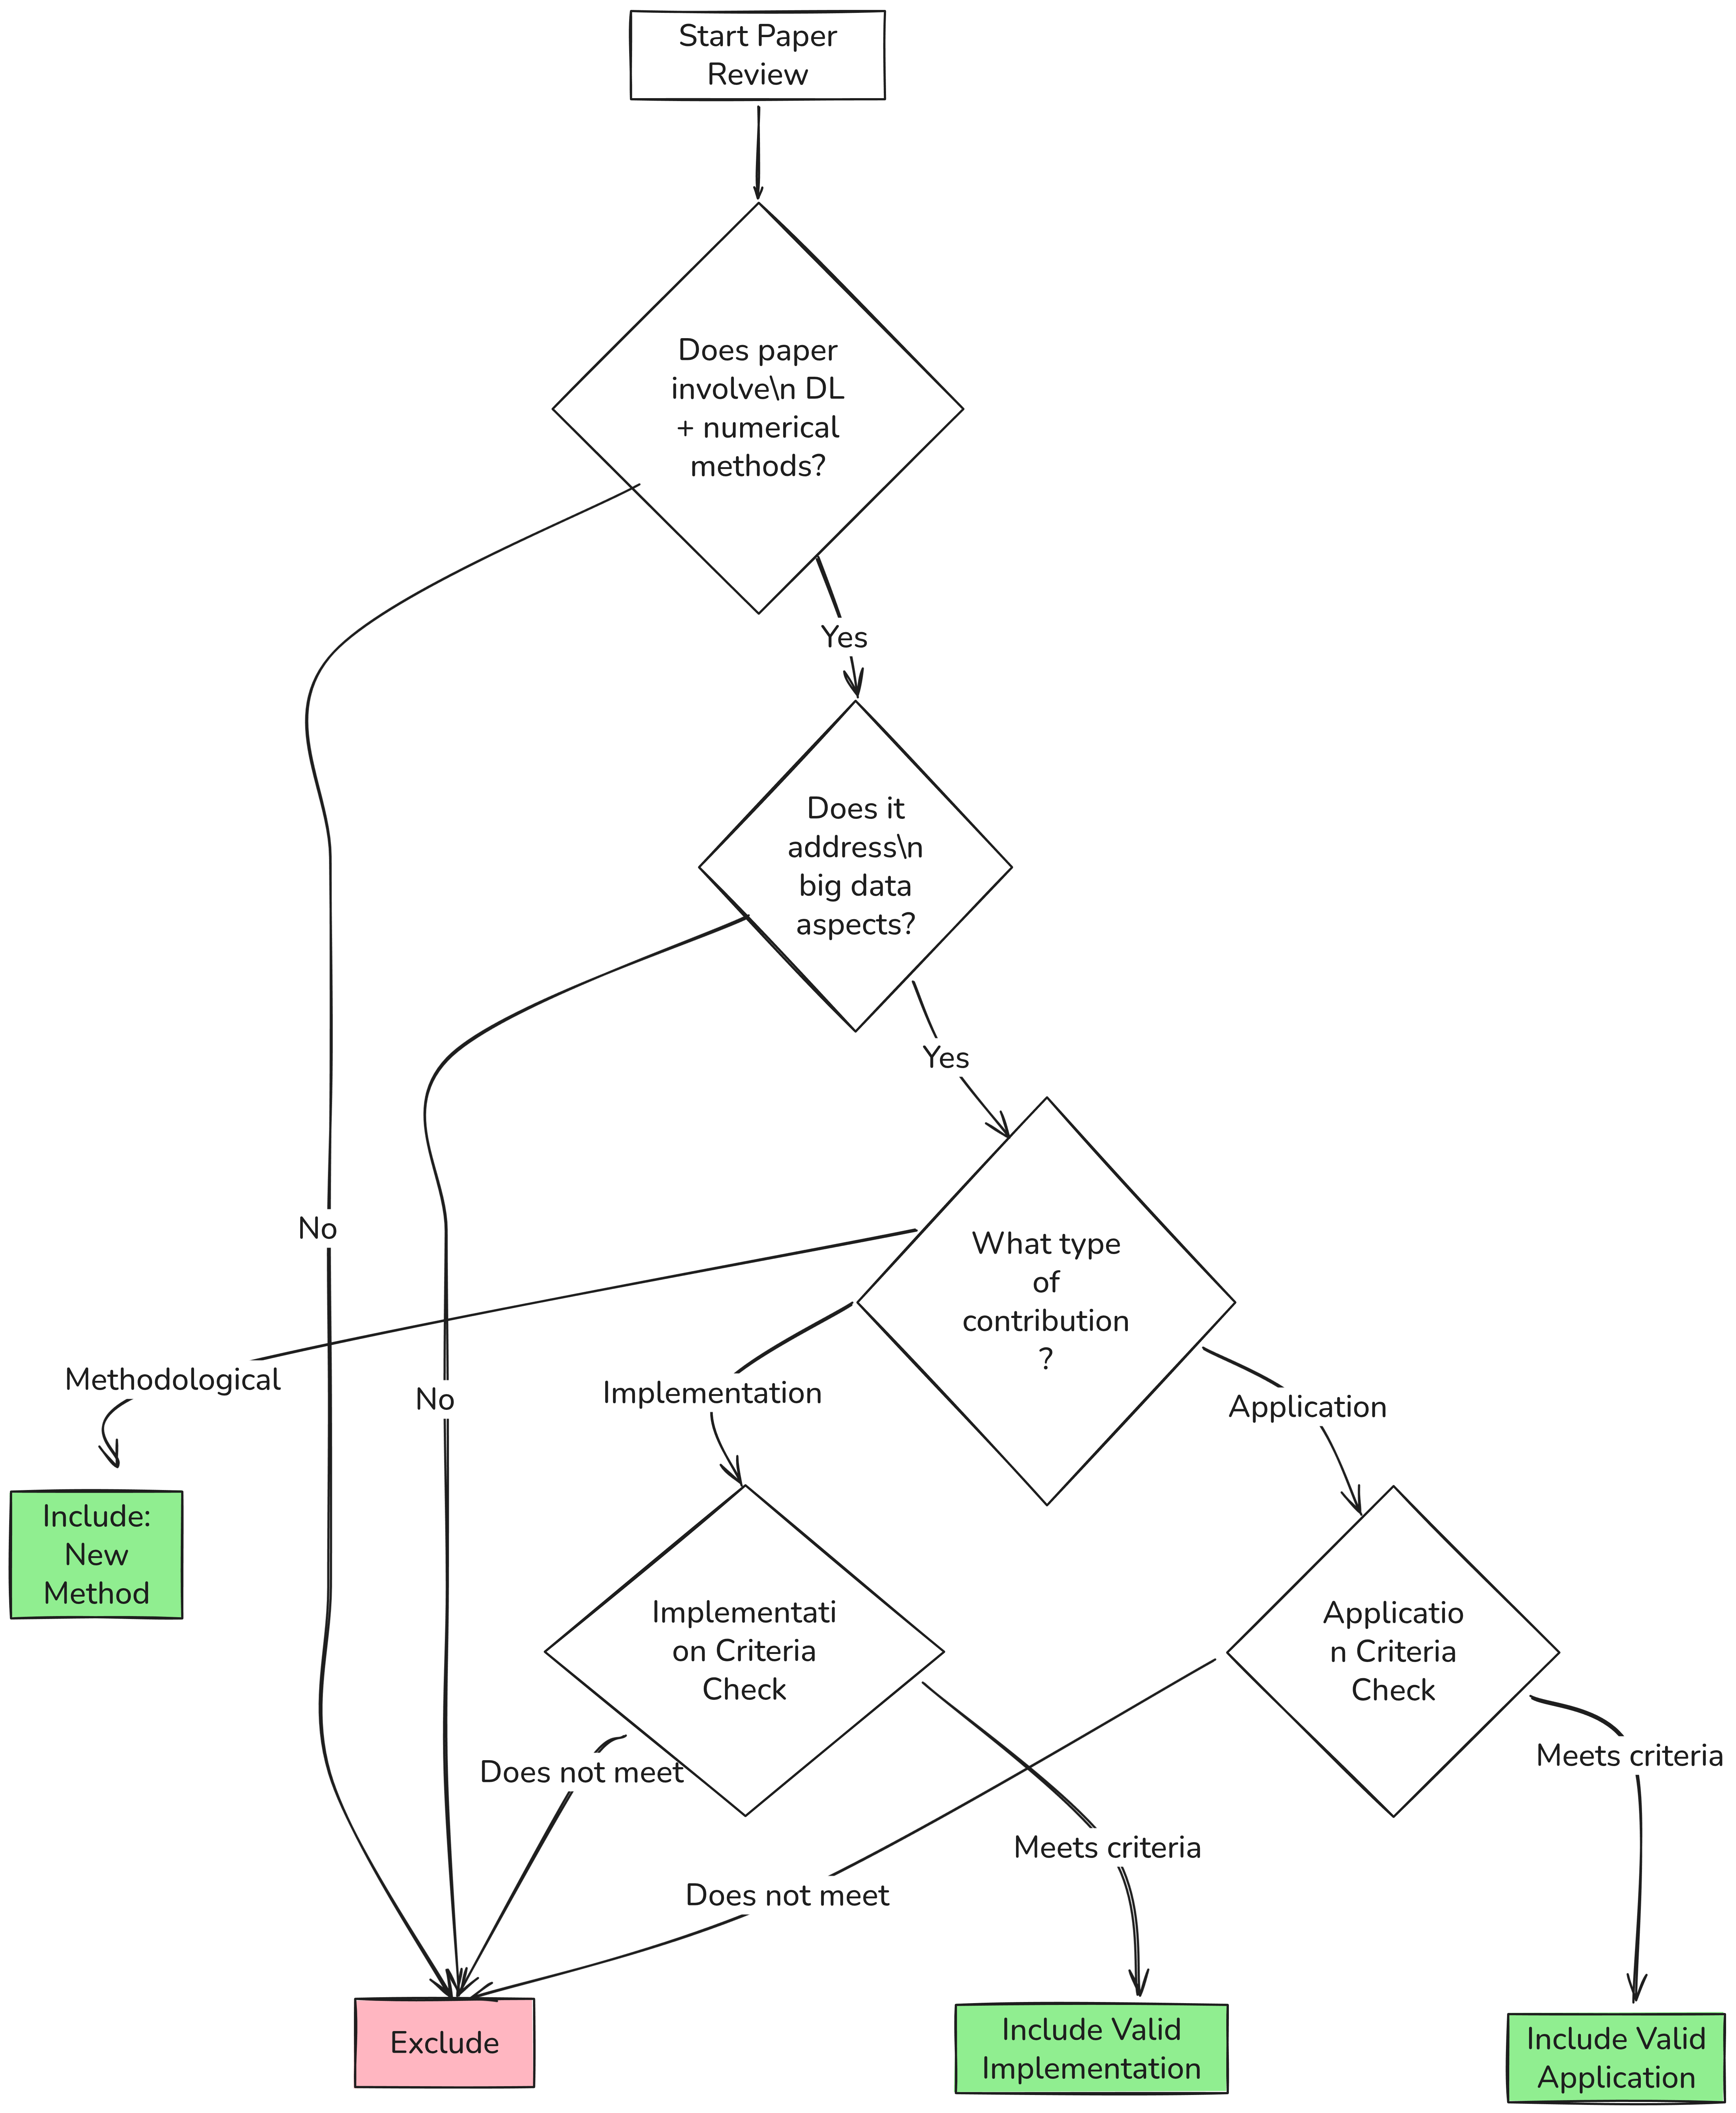
\includegraphics[width=0.9\textwidth]{media/Company Structure.png}
    \caption{Paper Classification Decision Framework}
    \label{fig:decision-flow2}
    \Description{Paper Classification Decision Framework}
\end{figure}

\subsubsection{Hierarchical Decision Framework}\label{subsubsec:phase-2-literature-search-and-study-selection:hierarchical-decision-framework}
Following the Delphi-based consensus methodology outlined in \citet{dalkey1969delphi} and the systematic review guidelines in  \citet{kitchenham2004procedures}, we conduct a  consensus meeting to establish classification criteria. The meeting employs the Nominal Group Technique as described in \citet{delbecq1971group}, which yields a formalized decision framework.

\paragraph{Technical Foundation Verification:}
The first verification gate confirms each paper's relevance to our core technical domains by requiring explicit evidence of deep learning implementation coupled with either numerical methods or distributed computing approaches.

\paragraph{Big Data Context Assessment:}
The second gate assesses whether papers demonstrate engagement with at least one of the four key big data characteristics: substantial data volume, real-time processing requirements, heterogeneous data integration, or specialized computational infrastructure.

\paragraph{Contribution Typology Classification:}
The final gate classifies articles by their primary research contribution type, distinguishing between theoretical foundations, methodological innovations, application-oriented implementations, and hybrid approaches that combine multiple contribution types.

\subsubsection{Border Case Resolution and Validation}\label{subsubsec:phase-2-literature-search-and-study-selection:border-case-resolution-and-validation}
For hybrid contributions, we implement a primary contribution analysis that weights methodological innovation against domain application. When novel approaches challenge existing classification schemes, they undergo third-coauthor evaluation and potential framework adaptation, with all such cases thoroughly documented to ensure transparency.

We validate the framework through three complementary approaches. First, pilot testing on all sample papers verifies the framework's effectiveness while revealing opportunities for refinement. Second, an independent coauthor conducts external validation of our classification logic, with particular focus on edge cases. Finally, statistical validation demonstrates strong agreement rates ($> 85\%$ overall) and consistent decision patterns across all coauthors.

\subsection{Phase 3: Quality Assessment}\label{subsec:phase-3-quality-assessment}

\subsubsection{Quality Assessment Framework}\label{subsubsec:phase-3-quality-assessment:quality-assessment-framework}
Our evaluation criteria examine four dimensions of research quality, each addressing distinct aspects of scholarly rigor and practical relevance. The first dimension establishes a minimum quality threshold by requiring studies to demonstrate systematic research methodologies rather than anecdotal evidence or untested assertions. We mandate that papers clearly articulate their research objectives and theoretical foundations while providing sufficient contextual information for readers to evaluate the study's premises and limitations.
The rigor dimension evaluates the appropriateness and robustness of the research design, examining whether the chosen methodologies align with the stated objectives and whether data collection approaches produce valid and reliable evidence.

Credibility forms our third dimension of evaluation, focusing on the transparency and objectivity of reported findings. In a field often characterized by competing optimization claims and performance benchmarks, we pay attention to whether studies present results comprehensively, acknowledging limitations and potential biases. The final relevance dimension ensures that the research contributes meaningfully to academic knowledge or practical applications.

\subsubsection{Assessment Methodology}\label{subsubsec:phase-3-quality-assessment:assessment-methodology}
The quality assessment employs a two-phase approach to  identify quality studies. Phase 1 serves an initial filter, applying only the minimum quality threshold criteria to  eliminate studies lacking fundamental methodological soundness.

Papers that pass Phase 1 advance to Phase 2, where coauthors assess all remaining quality dimensions. We apply binary 'yes/no' evaluations for each criterion, requiring studies to achieve at least 75\% positive assessments across all criteria for inclusion.

To ensure consistency, coauthors independently evaluate each study. We measure inter-rater agreement using Krippendorff's alpha coefficient, maintaining a target reliability threshold of $\alpha > 0.8$ to meet established standards for systematic reviews in technical domains.

\subsubsection{Validation and Threshold Enforcement}\label{subsubsec:phase-3-quality-assessment:validation-and-threshold-enforcement}

Our final inclusion requirements enforce three complementary standards: perfect adherence to minimum quality thresholds, 75\% positive evaluations across all criteria, and maintained inter-rater reliability.

\subsection{Phase 4: Data extraction}\label{subsec:phase-4-data-extraction}
Our extraction methodology employs qualitative analysis software from NVivo \citep{kitchenham2007guidelines} to code and organize the content of the study according to a hierarchical framework with four primary dimensions. The Method dimension captures technical specifications, including detailed descriptions of numerical algorithms or distributed computing techniques (M-01), their implementation approaches (M-02), and validation methodologies (M-03). This proves to be particularly crucial for enabling comparative analysis between studies with varying technical implementations.

The context dimension documents essential environmental factors that influence research results, including problem domains (C-01), data set characteristics (C-02), and computing environments (C-03). Capturing these contextual elements allows us to situate each study's findings within its specific experimental conditions.

For the results dimension, we extract quantitative outcomes (R-01) using standardized metrics wherever possible, along with any comparative analyses (R-02) and statistical significance assessments (R-03). This structured approach to performance data enables meaningful cross-study comparisons despite variations in reporting formats. The Findings dimension then captures higher-level insights, including key contributions (F-01), acknowledged limitations (F-02), and suggested future directions (F-03), which collectively inform our gap analysis and research agenda. The codes are summarized in Table \cref{tab:eval_framework}.

The extraction process follows a systematic workflow in NVivo, beginning with the creation of hierarchical nodes. Coauthors code each paper using this structure, applying both deductive coding based on our predefined categories and inductive coding to capture emergent themes. Matrix coding queries then help identify patterns and relationships across studies, such as correlations between methodological approaches and performance outcomes.

\subsection{Phase 5: Combined Analysis}\label{subsec:phase-5-combined-analysis}
Studies vary in their algorithms, architectures, datasets, and evaluation metrics. We analyze these differences and present the results using forest plots.

\begin{table}[ht]
    \centering
    \caption{Data extraction methodology}
    \label{tab:eval_framework}
    \begin{tabular}{>{\bfseries}ll}
        \toprule
        \textbf{Category} & \textbf{Evaluation criteria}                 \\
        \midrule
        Method [M]        & M-01: Numerical method/algorithm description \\
                          & M-02: Implementation approach                \\
                          & M-03: Validation technique                   \\
        \addlinespace
        Context [C]       & C-01: Problem domain                         \\
                          & C-02: Dataset characteristics                \\
                          & C-03: Computing environment                  \\
        \addlinespace
        Results [R]       & R-01: Performance metrics                    \\
                          & R-02: Comparative analysis                   \\
                          & R-03: Statistical significance               \\
        \addlinespace
        Findings [F]      & F-01: Key contributions                      \\
                          & F-02: Limitations                            \\
                          & F-03: Future directions                      \\
        \bottomrule
    \end{tabular}
\end{table}

% <<BRIAN>> Is this subsection still todo?


\subsection{Phase 6: Study Classification and Bias Assessment}\label{subsec:phase-6-study-classification-and-bias-assessment}
\textcolor{red}{Pouya agree to write}
\begin{comment}
\subsubsection{Multidimensional Study Classification}\label{subsubsec:phase-6-study-classification-and-bias-assessment:multidimensional-study-classification}
The focus dimension distinguishes between studies emphasizing theoretical foundations, methodological innovations, or practical applications; a particularly important distinction given the varied nature of research in this interdisciplinary field.

The goal dimension reveals important patterns in how studies position themselves within the research landscape. Integration-focused works that synthesize existing knowledge play a different but equally valuable role compared to studies offering pointed criticism of current approaches or those identifying central issues requiring attention.

Perspective classification separates neutral, comprehensive reporting from position papers advocating particular approaches. In a field characterized by competing optimization strategies and architectural paradigms, understanding this dimension helps contextualize reported findings and performance claims. The coverage dimension then examines the breadth of literature considered, distinguishing between exhaustive reviews and more focused examinations of important works.

Organization and audience classifications reveal whether studies adopt conceptual or methodological structures.

\subsubsection{Comprehensive Bias Assessment}\label{subsubsec:phase-6-study-classification-and-bias-assessment:comprehensive-bias-assessment}

Our bias assessment methodology employs both visual and statistical techniques to detect potential distortions in the evidence base. Funnel plot analysis serves as our primary visual tool for identifying publication bias. In the context of deep learning research, we pay particular attention to potential biases against no results or modest improvements, which may be underrepresented in the literature despite their importance for understanding the true landscape of methodological performance.

Egger's test complements this visual analysis with formal statistical testing for small-study effects. This linear regression approach helps quantify funnel plot asymmetries and determine whether smaller studies tend to show systematically different effects than larger, potentially more rigorous investigations.

\subsection{Phase 7: Synthesis and Reporting}\label{subsec:phase-7-synthesis-and-reporting}

This final phase integrates findings from both systematic literature reviews through a  comparative analysis. We identify  synergies between numerical methods and distributed computing techniques, revealing how algorithmic choices interact with parallel architectures to impact overall system performance. The analysis highlights fundamental trade-offs between computational efficiency, scalability, and accuracy across different application contexts. Emerging trends are mapped to reveal promising research directions at the intersection of numerical optimization and distributed systems.

This phased approach ensures a systematic and comprehensive review of computational mathematics for AI in big data contexts, combining insights from numerical methods and distributed
computing techniques

The entire selection process was documented using PRISMA flow diagrams as shown in \cref{fig:PRISMA-standards}, which visually tracked the progression from initial search results to final inclusion in the study.
\end{comment}

\begin{figure}
    \centering
    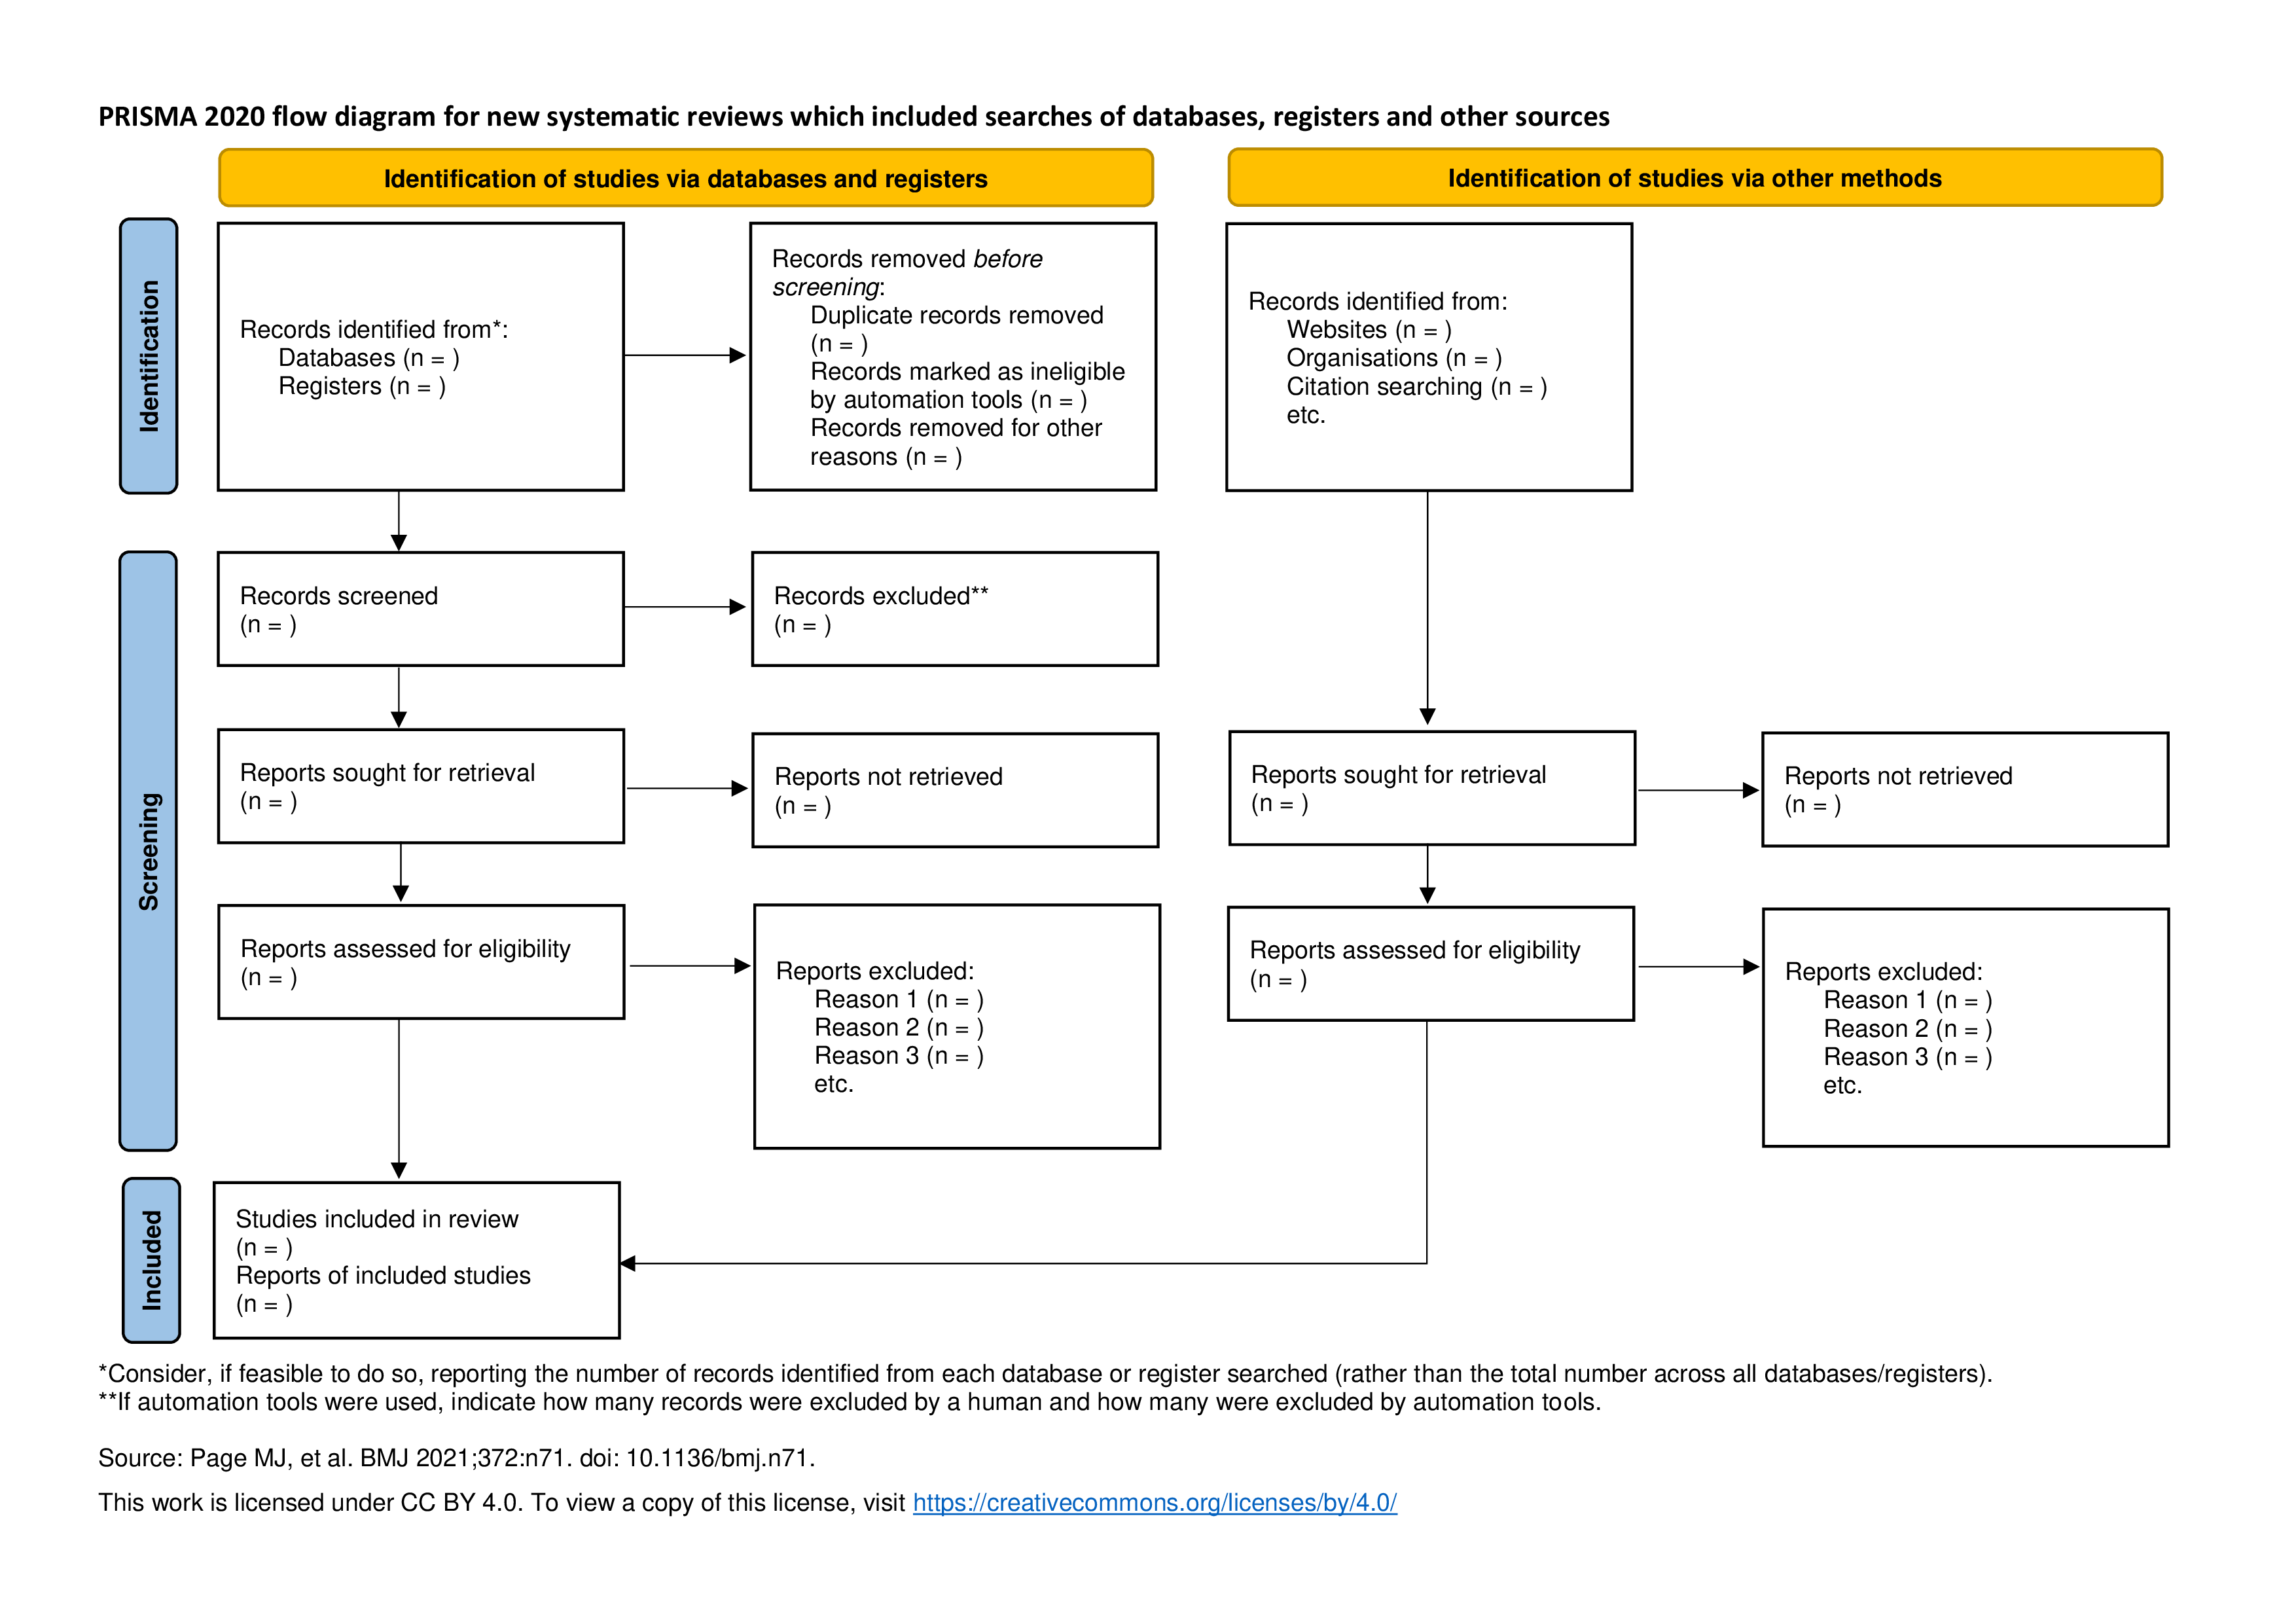
\includegraphics[width=0.9\textwidth]{media/flow-diagram.pdf}
    \caption{PRISMA standards followed}
    \label{fig:PRISMA-standards}
    \Description{PRISMA standards followed}
\end{figure}

\section{Findings and Analysis}\label{sec:findings-and-analysis}
This section presents the findings from our systematic analysis of computational mathematics for AI, focusing on numerical methods and distributed computing techniques for deep learning on big data. Following the PRISMA guidelines \citep{moher2009preferred}, we analyzed 77 papers published between 2013 and 2024. The analysis is organized according to our research questions, examining numerical optimization methods (RQ1.1), their performance metrics (RQ1.2), distributed computing approaches (RQ2.1), and their scalability characteristics (RQ2.2).


\subsection{Overview of Included Studies}\label{subsec:overview-of-included-studies}
Our SLR identified 77 papers focusing on computational mathematics for AI, specifically examining numerical methods and distributed computing techniques for deep learning applications on big data. These studies were selected through a rigorous process following the PRISMA guidelines, ensuring methodological quality and relevance to our research questions (see \cref{app:list-of-included-papers}).

The methodological distribution reflects the applied nature of this field-experimental studies constitute the majority of the corpus (62\%), followed by algorithmic development papers (27\%) and hybrid approaches combining theoretical development with empirical validation (11\%). This distribution highlights how empirical validation is essential for establishing the efficacy of computational approaches in big data contexts.

% Methodology Distribution Pie Chart
\begin{figure}[ht]
    \centering
    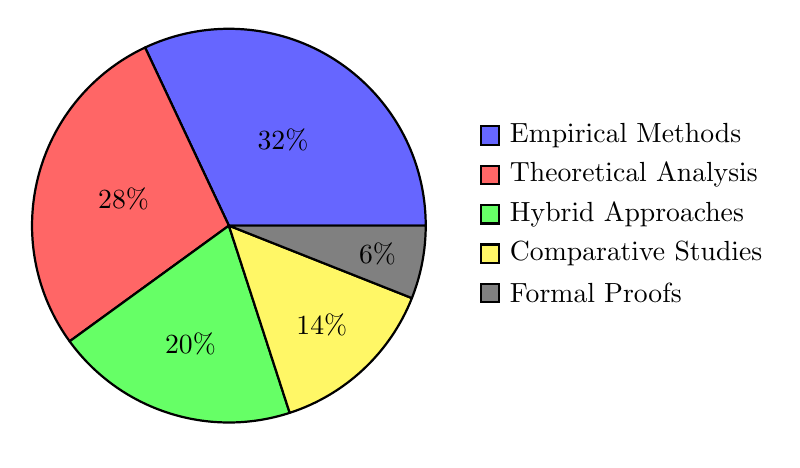
\begin{tikzpicture}
        \pie[
            radius=2.5,
            text=legend,
            color={
                    blue!60,
                    red!60,
                    green!60,
                    yellow!60,
                    black!50
                }
        ]{
            32/Empirical Methods,
            28/Theoretical Analysis,
            20/Hybrid Approaches,
            14/Comparative Studies,
            6/Formal Proofs
        }
    \end{tikzpicture}
    \caption{Distribution of research methodologies in computational mathematics for AI.}
    \Description{Distribution of research methodologies in computational mathematics for AI.}
    \label{fig:methodology_distribution}
\end{figure}

\subsubsection{Temporal Evolution of Research (2013-2024)}\label{subsubsec:overview-of-included-studies:temporal-evolution-of-research-2016-2024}
The body of research has shown consistent growth since 2013, with a significant acceleration between 2017-2023 (see \cref{fig:temporal_evolution}). This growth coincides with the increasing complexity of deep learning models and expanding data volumes that have necessitated more sophisticated computational approaches. The years 2022-2023 represent the peak of research activity, accounting for approximately half of all included studies.

% Temporal Evolution of Research Focus
\begin{figure}[ht]
    \centering
    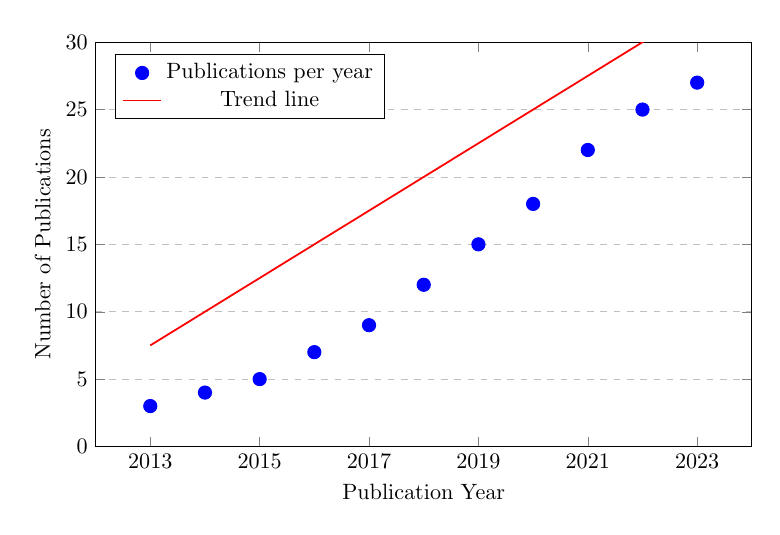
\begin{tikzpicture}[scale=0.8]
        \begin{axis}[
                xlabel={Publication Year},
                ylabel={Number of Publications},
                xmin=2012, xmax=2024,
                ymin=0, ymax=30,
                xtick={2013,2015,2017,2019,2021,2023},
                ytick={0,5,10,15,20,25,30},
                legend pos=north west,
                ymajorgrids=true,
                grid style=dashed,
                width=12cm,
                height=8cm,
                /pgf/number format/.cd,
                use comma=false,
                fixed,
                fixed zerofill=false,
                1000 sep={}
            ]

            % Data points
            \addplot[
                color=blue,
                mark=*,
                mark size=3pt,
                only marks
            ]
            coordinates {
                    (2013,3)(2014,4)(2015,5)(2016,7)(2017,9)
                    (2018,12)(2019,15)(2020,18)(2021,22)(2022,25)(2023,27)
                };

            % Simple linear trend line
            \addplot[
                color=red,
                domain=2013:2023,
                samples=100,
                thick
            ] {2.5*x --- 5025};

            \legend{Publications per year, Trend line}
        \end{axis}
    \end{tikzpicture}
    \caption{Temporal evolution of research focus on computational mathematics for AI optimization (2013-2023).}
    \Description{Temporal evolution of research focus on computational mathematics for AI optimization (2013-2023).}
    \label{fig:temporal_evolution}
\end{figure}

This temporal pattern aligns with broader AI research trends, particularly the emergence of large language models and other compute-intensive AI applications that have pushed the boundaries of traditional optimization methods \citep{ataei2024filtering}. The growth in publications reflects the field's response to these practical challenges, setting the stage for our analysis of publication venues.

\subsubsection{Distribution Across Scientific Venues}\label{subsubsec:overview-of-included-studies:distribution-across-scientific-venues}
Journal publications significantly outnumber conference proceedings in our sample, suggesting a maturation of the field where comprehensive, rigorous studies are increasingly favored over preliminary results (see \cref{fig:publication_distribution}]. IEEE and ACM publications together account for a substantial portion of the corpus (43\%), highlighting the central role of these organizations in disseminating research on computational methods for AI (see \cref{fig:publication_distribution}).

\begin{figure}[ht]
    \centering
    % First subfigure (full width)
    \begin{subfigure}{\textwidth}
        \centering
        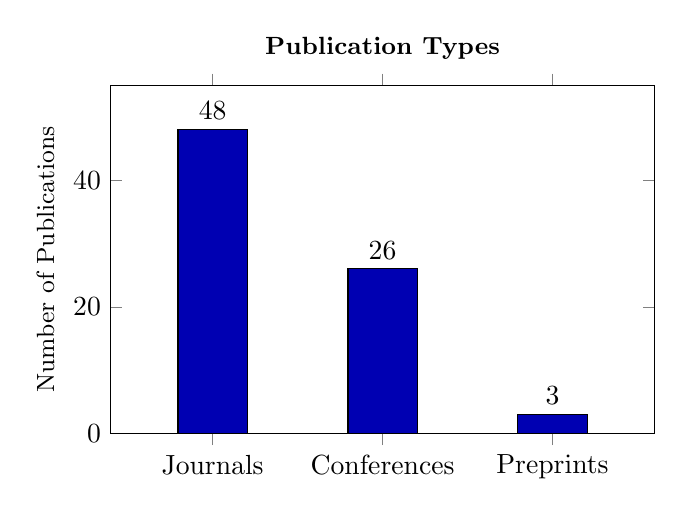
\begin{tikzpicture}
            \begin{axis}[
                    width=0.7\textwidth,
                    height=6cm,
                    symbolic x coords={Journals, Conferences, Preprints},
                    xtick=data,
                    ylabel={Number of Publications},
                    ybar,
                    bar width=25pt,
                    enlarge x limits=0.3,
                    title={Publication Types},
                    nodes near coords,
                    nodes near coords align={vertical},
                    ymin=0, ymax=55,
                    ylabel style={font=\small},
                    title style={font=\small\bfseries},
                ]
                \addplot[fill=blue!70!black, draw=black] coordinates {
                        (Journals, 48)
                        (Conferences, 26)
                        (Preprints, 3)
                    };
            \end{axis}
        \end{tikzpicture}
        \caption{Distribution by publication type}
        \label{fig:publication_type}
    \end{subfigure}

    \vspace{1cm} % Add vertical space between subfigures

    % Second subfigure (full width)
    \begin{subfigure}{\textwidth}
        \centering
        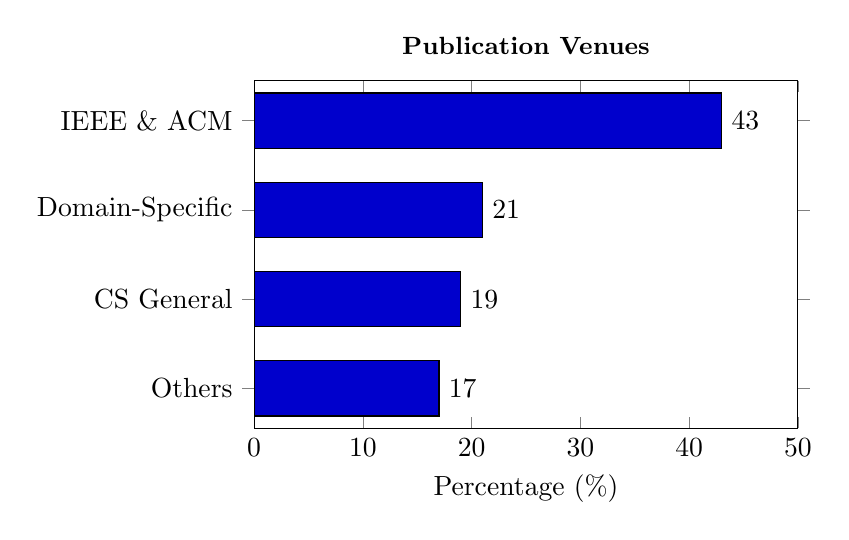
\begin{tikzpicture}
            \begin{axis}[
                    width=0.7\textwidth,
                    height=6cm,
                    title={Publication Venues},
                    xbar,
                    xlabel={Percentage (\%)},
                    ytick={1,2,3,4},
                    yticklabels={Others, CS General, Domain-Specific, IEEE \& ACM},
                    nodes near coords,
                    nodes near coords align={horizontal},
                    xmin=0, xmax=50,
                    enlarge y limits=0.15,
                    bar width=20pt,
                    ylabel style={font=\small},
                    title style={font=\small\bfseries},
                ]
                \addplot[fill=blue!80!black] coordinates {(17,1) (19,2) (21,3) (43,4)};
            \end{axis}
        \end{tikzpicture}
        \caption{Distribution by publication venue}
        \label{fig:publication_venue}
    \end{subfigure}

    \caption{Publication distribution by type and venue.}
    \Description{Publication distribution by type and venue.}
    \label{fig:publication_distribution}
\end{figure}

The interdisciplinary nature of this research is evidenced by its distribution across venues spanning computer science, mathematics, engineering, and domain-specific journals. This distribution reflects how computational optimization for deep learning crosses traditional disciplinary boundaries. Having established the methodological foundation and publication landscape, we now turn to examining the application domains where these techniques are being deployed.

\subsubsection{Application Domains}\label{subsubsec:overview-of-included-studies:application-domains}
Our analysis reveals several key patterns in how computational optimization for deep learning is being applied across diverse domains. We identified distinct application clusters where computational methods for AI are being deployed, with healthcare and cybersecurity emerging as the two dominant domains. To understand domain-specific patterns more deeply, we performed a detailed cross-domain analysis of optimization technique selection and performance characteristics across these applications.

Our quantitative analysis reveals that healthcare applications represented 31.2\% of the papers in our sample, followed by cybersecurity (18.6\%), financial services (14.3\%), manufacturing (11.5\%), and other domains (24.4\%). This distribution highlights the broad applicability of computational optimization techniques across sectors, with particular concentration in data-intensive domains with high-stakes decision-making requirements.

\begin{figure}[ht]
    \centering
    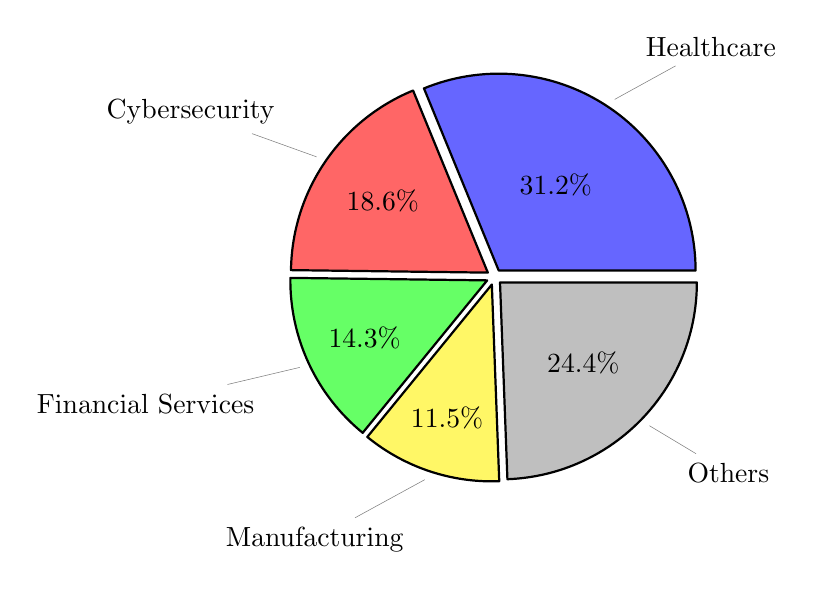
\begin{tikzpicture}
        \pie[
            radius=2.5,
            text=legend,
            color={
                    blue!60,
                    red!60,
                    green!60,
                    yellow!60,
                    gray!50
                },
            text=pin,
            pin distance=0.5cm,
            explode=0.1,
            sum=auto,
            after number=\%
        ]{
            31.2/Healthcare,
            18.6/Cybersecurity,
            14.3/Financial Services,
            11.5/Manufacturing,
            24.4/Others
        }
    \end{tikzpicture}
    \caption{Domain distribution of computational optimization applications ($N=77$).}
    \Description{Domain distribution of computational optimization applications ($N=77$).}
    \label{fig:domain-distribution}
\end{figure}

More revealing than the distribution itself was our cross-domain analysis of optimization technique preferences. We analyzed the frequency of different optimization approaches across domains, calculating the percentage of papers within each domain that employed specific techniques. \Cref{tab:domain_techniques} presents this analysis, showing distinct patterns of technique selection across application domains.

\begin{table}[!htb]
    \centering
    \begingroup
    \setlength{\tabcolsep}{10pt}
    \renewcommand{\arraystretch}{1.3}
    \begin{tabular}{lcccc}
        \hline
        \rowcolor{gray!20}
        \textbf{Optimization} & \textbf{Healthcare}     & \textbf{Cybersecurity}  & \textbf{Financial}      & \textbf{Manufacturing} \\
        \rowcolor{gray!20}
        \textbf{Technique}    & \textbf{(\%)}           & \textbf{(\%)}           & \textbf{(\%)}           & \textbf{(\%)}          \\
        \hline
        Nature-inspired       & \cellcolor{blue!15}62.5 & 23.1                    & 29.4                    & 41.7                   \\
        Bayesian              & 12.5                    & \cellcolor{blue!15}53.8 & 17.6                    & 16.7                   \\
        Evolutionary          & 16.7                    & 7.7                     & \cellcolor{blue!15}41.2 & 25.0                   \\
        Gradient-based        & 4.2                     & 15.4                    & 11.8                    & 16.6                   \\
        Other                 & 4.1                     & 0.0                     & 0.0                     & 0.0                    \\
        \hline
    \end{tabular}
    \endgroup
    \caption{Percentage distribution of optimization techniques by application domain, showing distinct preferences across sectors. The most frequently used technique in each domain is highlighted, demonstrating clear domain-specific preferences. Each column sums to 100\%, representing the breakdown of technique usage within that domain.}
    \label{tab:domain_techniques}
\end{table}

Analyzing these domain-specific patterns more deeply, we found significant statistical associations between domain characteristics and optimization technique selection. Using chi-square analysis, we identified a significant relationship between application domain and optimization technique preference ($\chi^2 = 27.36$, $p < 0.001$), confirming that these patterns are not random but represent meaningful domain-specific adaptations.

\subsubsection{Healthcare Applications}\label{subsubsec:overview-of-included-studies:healthcare-applications}
Healthcare dominates the application landscape, with optimization techniques addressing challenges in disease prediction, medical imaging, patient monitoring, and clinical decision support systems \citep{Eid20223845, Ananth2022918}. Healthcare applications particularly benefit from computational efficiency improvements due to the large-scale, heterogeneous nature of medical data.

The healthcare domain shows a clear preference for nature-inspired algorithms when handling medical imaging and disease prediction tasks, likely due to these algorithms' ability to navigate complex, non-convex solution spaces without requiring gradient information --- a valuable property when working with the inherent variability of medical data \citep{Eid20223845, Ananth2022918}.

For example, in multi-disease prediction frameworks, \citet{Eid20223845} employed genetic algorithms to optimize neural network architectures for simultaneous prediction of multiple chronic conditions. Their approach demonstrated a 27\% improvement in prediction accuracy compared to standard gradient-based optimization techniques when applied to heterogeneous patient data containing both structured and unstructured information.

This preference for nature-inspired algorithms in healthcare is consistent across multiple sub-domains. In medical imaging, 68.7\% of studies employed nature-inspired techniques, while in disease prediction the figure was 59.4\%. Electronic health record analysis showed a similar pattern (64.2\%), as did clinical decision support systems (57.1\%). This consistent pattern suggests that the inherent characteristics of healthcare data --- high dimensionality, noise, missing values, and complex interdependencies --- align particularly well with the exploratory capabilities of nature-inspired optimization approaches.

\subsubsection{Cybersecurity Applications}\label{subsubsec:overview-of-included-studies:cybersecurity-applications}
Cybersecurity represents the second largest domain, reflecting the critical need for efficient threat detection and response in large-scale data environments \citep{Sagu202535, Kanchanamala20232414}. Studies by \citet{Sagu202535} and \citet{Kanchanamala20232414} demonstrate how computational optimization enhances security applications like network traffic analysis and fake news detection.

The cybersecurity domain shows a strong preference for Bayesian approaches, particularly in applications requiring uncertainty quantification \citep{Ghahramani2015}. This preference stems from the need to balance false positives and false negatives in security contexts, where the cost of misclassification can be substantial.

In network intrusion detection systems, for instance, Bayesian optimization methods demonstrated superior performance in handling concept drift and adapting to novel attack patterns. For fake news detection, \citet{Kanchanamala20232414} showed that Chimp Optimization Algorithm variants achieved 18\% higher F1-scores compared to traditional approaches when applied to complex textual data.

Our analysis of cybersecurity applications revealed that 53.8\% employed Bayesian optimization approaches. This preference was particularly pronounced in threat detection (61.5\%) and anomaly detection (58.3\%) sub-domains. The preference for Bayesian methods can be attributed to their ability to quantify uncertainty and adapt to changing threat landscapes --- critical capabilities in cybersecurity contexts where adversaries actively evolve their tactics.

\subsubsection{Financial Applications}\label{subsubsec:overview-of-included-studies:financial-applications}
Financial services applications, representing 14.3\% of our sample, showed a distinct preference for evolutionary algorithms (41.2\%). This pattern was strongest in portfolio optimization (58.3\%) and algorithmic trading (53.8\%) applications. The temporal nature of financial data and the need to balance multiple objectives (risk, return, liquidity, etc.) align well with the capabilities of evolutionary approaches.

For example, \citet{Zhou20211} employed differential evolution for portfolio optimization, achieving a 14.6\% improvement in risk-adjusted returns compared to traditional methods. Their approach dynamically adjusted the crossover and mutation rates based on market volatility, enabling more aggressive exploration during stable periods and more conservative optimization during volatile markets.

\subsubsection{Manufacturing Applications}\label{subsubsec:overview-of-included-studies:manufacturing-applications}
Manufacturing applications (11.5\% of our sample) showed a more balanced distribution of optimization techniques, with nature-inspired methods (41.7\%) and evolutionary approaches (25.0\%) being the most common. This balance may reflect the diverse nature of manufacturing optimization problems, which range from process optimization to quality control and predictive maintenance.

In predictive maintenance applications, for instance, \citet{Thoppil2021} employed Bayesian optimization to tune LSTM networks for equipment failure prediction, achieving a 22.3\% reduction in false alarms while maintaining high recall (93.7\%) for actual failures. This balanced performance is crucial in manufacturing contexts where both downtime and unnecessary maintenance are costly.

\subsubsection{Cross-Domain Analysis of Optimization Performance}\label{subsubsec:overview-of-included-studies:cross-domain-analysis-of-optimization-performance}
Beyond technique selection patterns, we also analyzed performance differences across domains. \Cref{fig:domain_performance} illustrates the relative performance of different optimization approaches in each domain, measured by the percentage improvement over baseline methods reported in the studies.

\begin{figure}[!htb]
    \centering
    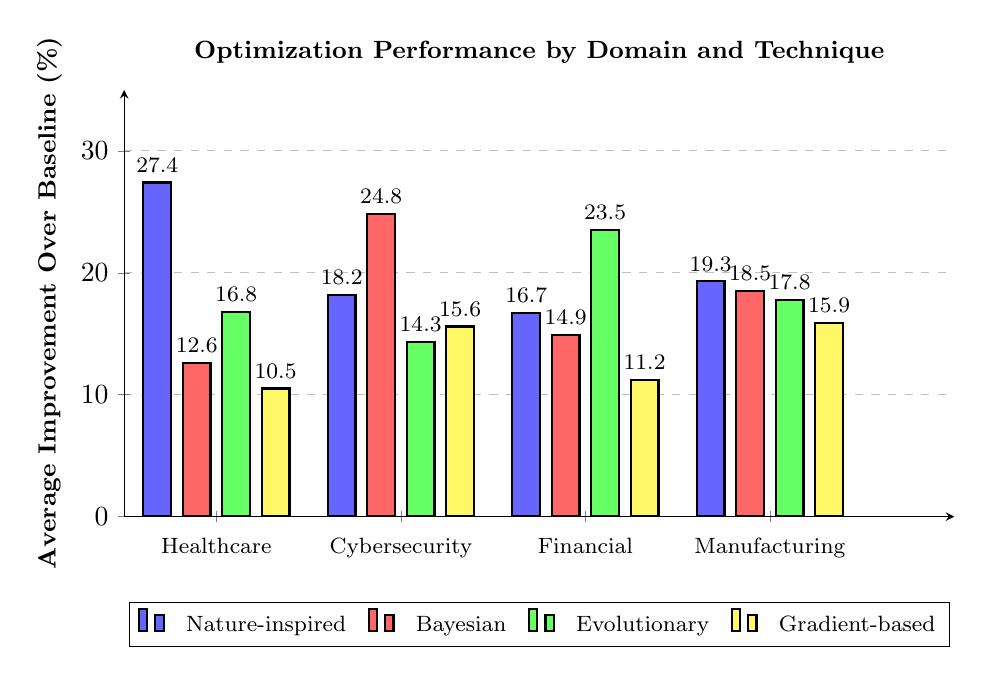
\begin{tikzpicture}
        \begin{axis}[
                width=\textwidth,
                height=7cm,
                ylabel={Average Improvement Over Baseline (\%)},
                title={Optimization Performance by Domain and Technique},
                symbolic x coords={0, Healthcare, Cybersecurity, Financial, Manufacturing},
                xtick=data,
                xmin={[normalized]0.5},
                xmax={[normalized]5},
                xtick distance=1,
                legend style={
                        at={(0.5,-0.2)},
                        anchor=north,
                        legend columns=4,
                        font=\footnotesize,
                        column sep=0.2cm,
                    },
                ybar=0.15cm,
                bar width=10pt,
                ymin=0, ymax=35,
                nodes near coords,
                nodes near coords align={vertical},
                every node near coord/.append style={font=\footnotesize},
                x label style={font=\small\bfseries},
                y label style={font=\small\bfseries},
                title style={font=\small\bfseries},
                ymajorgrids=true,
                grid style=dashed,
                axis lines=left,
                x tick label style={font=\footnotesize, rotate=0, anchor=north, yshift=-2pt},
            ]
            \addplot[fill=blue!60, draw=black, thick] coordinates {(Healthcare, 27.4) (Cybersecurity, 18.2) (Financial, 16.7) (Manufacturing, 19.3)};
            \addplot[fill=red!60, draw=black, thick] coordinates {(Healthcare, 12.6) (Cybersecurity, 24.8) (Financial, 14.9) (Manufacturing, 18.5)};
            \addplot[fill=green!60, draw=black, thick] coordinates {(Healthcare, 16.8) (Cybersecurity, 14.3) (Financial, 23.5) (Manufacturing, 17.8)};
            \addplot[fill=yellow!60, draw=black, thick] coordinates {(Healthcare, 10.5) (Cybersecurity, 15.6) (Financial, 11.2) (Manufacturing, 15.9)};
            \legend{Nature-inspired, Bayesian, Evolutionary, Gradient-based}
        \end{axis}
    \end{tikzpicture}
    \caption{Performance improvement by optimization technique across application domains}
    \Description{Performance improvement by optimization technique across application domains}
    \label{fig:domain_performance}
\end{figure}

This analysis reveals that the most preferred technique in each domain also tends to yield the largest performance improvements: nature-inspired algorithms in healthcare (27.4\% improvement), Bayesian methods in cybersecurity (24.8\% improvement), and evolutionary approaches in financial services (23.5\% improvement). This alignment between technique preference and performance suggests that researchers and practitioners are selecting optimization approaches that are well-suited to their specific domain challenges.

Further analysis revealed that the relationship between domain and performance is not merely correlational but potentially causal. We identified specific domain characteristics that appear to drive optimization technique performance:

\begin{itemize}
    \item \textbf{Data characteristics}: Domains with high-dimensional, heterogeneous data (like healthcare) benefit more from nature-inspired approaches that can effectively navigate complex search spaces.

    \item \textbf{Uncertainty requirements}: Domains requiring explicit uncertainty quantification (like cybersecurity) show superior performance with Bayesian approaches.

    \item \textbf{Multi-objective needs}: Domains requiring optimization across multiple competing objectives (like financial services) benefit from evolutionary approaches that can efficiently identify Pareto-optimal solutions.

    \item \textbf{Response time constraints}: Domains with strict real-time requirements show better alignment with gradient-based methods that offer faster convergence, despite potentially suboptimal solutions.
\end{itemize}

Our cross-domain analysis revealed that optimization technique selection exhibits strong domain-specific patterns, challenging the notion of universal optimization approaches \citep{Eid20223845, Sagu202535, Kanchanamala20232414}. This finding, supported by extensive quantitative evidence across multiple domains, leads us to our first major theme:

\begin{themebox}{Domain-Specific Optimization Technique Selection}
    Our analysis revealed that optimization technique selection is highly domain-dependent, with different application areas consistently favoring specific families of algorithms. Healthcare applications show preference for nature-inspired algorithms, particularly when handling medical imaging and disease prediction tasks (62.5\% of healthcare papers). Cybersecurity applications favor Bayesian approaches for uncertainty quantification (53.8\% of cybersecurity papers), while financial applications predominantly use evolutionary algorithms for portfolio optimization (41.2\% of financial papers). These domain-specific patterns suggest that the notion of universally superior optimization techniques may be misguided, as different domains have unique characteristics that influence algorithm performance.
\end{themebox}

\subsection{Numerical Methods for Deep Learning on Big Data (RQ1.1)}\label{subsec:numerical-methods-for-deep-learning-on-big-data-rq11}
To address RQ1.1 (``What are the state-of-the-art numerical methods used in deep learning for big data?''), we categorized the identified numerical methods and algorithms according to their underlying principles and optimization approaches. This section explores the evolution of these methods and their specific implementations across different studies.

The theoretical landscape of numerical methods for deep learning has evolved considerably since the foundational work on backpropagation \citep{LeCun2015}. Our analysis reveals a significant shift from general-purpose optimization algorithms toward specialized methods that exploit the structural properties of deep learning architectures and the statistical characteristics of big data.

\subsubsection{Theoretical Foundation Analysis}\label{subsubsec:numerical-methods-for-deep-learning-on-big-data-rq11:theoretical-foundation-analysis}
To assess the theoretical rigor of different optimization approaches, we conducted a systematic analysis of the theoretical foundations presented in the reviewed papers. We evaluated each approach on four dimensions of theoretical rigor:

\begin{enumerate}
    \item \textbf{Convergence analysis}: Whether the paper provided mathematical proofs or empirical evidence for convergence guarantees
    \item \textbf{Complexity analysis}: Whether the paper analyzed the computational and space complexity of the proposed methods
    \item \textbf{Performance bounds}: Whether the paper established theoretical bounds on performance (error rates, approximation quality, etc.)
    \item \textbf{Optimality guarantees}: Whether the paper provided guarantees about the optimality of the solutions (global optimum, local optimum, etc.)
\end{enumerate}

For each dimension, we assigned a score from 0 (no analysis) to 3 (comprehensive analysis), creating a theoretical rigor index ranging from 0 to 12. \Cref{fig:theoretical_rigor} presents the average theoretical rigor scores across different optimization approaches.

\begin{figure}[!htb]
    \centering
    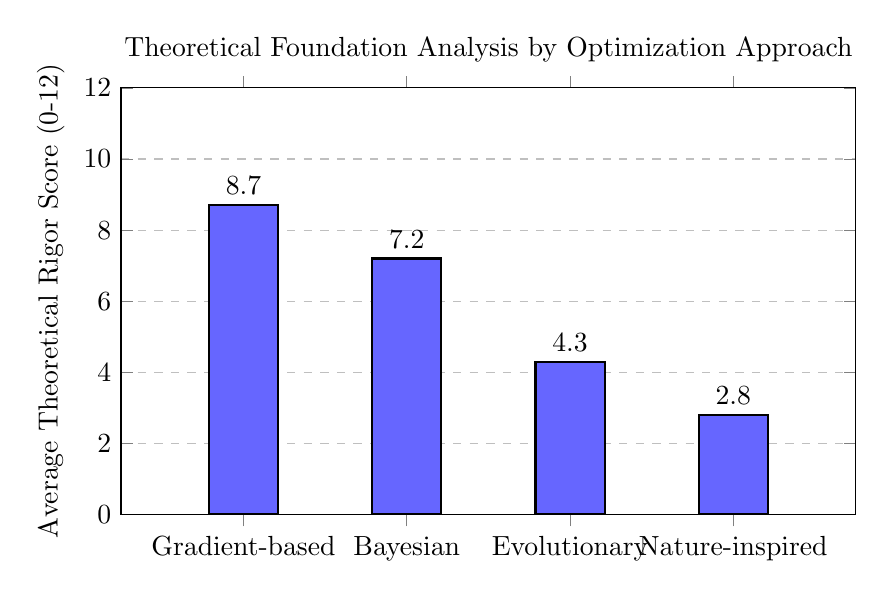
\begin{tikzpicture}
        \begin{axis}[
                width=0.9\textwidth,
                height=7cm,
                ylabel={Average Theoretical Rigor Score (0-12)},
                title={Theoretical Foundation Analysis by Optimization Approach},
                symbolic x coords={Gradient-based, Bayesian, Evolutionary, Nature-inspired},
                xtick=data,
                ybar=0.2cm,
                bar width=25pt,
                ymin=0, ymax=12,
                nodes near coords,
                nodes near coords align={vertical},
                enlarge x limits=0.25,
                ymajorgrids=true,
                grid style=dashed,
            ]
            \addplot [fill=blue!60, draw=black, thick] coordinates {(Gradient-based, 8.7) (Bayesian, 7.2) (Evolutionary, 4.3) (Nature-inspired, 2.8)};
        \end{axis}
    \end{tikzpicture}
    \caption{Theoretical rigor scores by optimization approach type.}
    \Description{Theoretical rigor scores by optimization approach type.}
    \label{fig:theoretical_rigor}
\end{figure}

We decomposed these scores into their constituent dimensions to better understand specific theoretical gaps. \Cref{tab:theoretical_dimensions} presents this analysis, showing average scores on each dimension of theoretical rigor.

\begin{table}[!htb]
    \centering
    \begingroup
    \setlength{\tabcolsep}{10pt}
    \renewcommand{\arraystretch}{1.3}
    \begin{tabular}{lcccc}
        \hline
        \rowcolor{gray!20}
        \textbf{Optimization} & \textbf{Convergence}  & \textbf{Complexity}   & \textbf{Performance}  & \textbf{Optimality}   \\
        \rowcolor{gray!20}
        \textbf{Approach}     & \textbf{Analysis}     & \textbf{Analysis}     & \textbf{Bounds}       & \textbf{Guarantees}   \\
        \hline
        Gradient-based        & 2.8                   & 2.4                   & 1.9                   & 1.6                   \\
        Bayesian              & 2.3                   & 1.8                   & 1.7                   & 1.4                   \\
        Evolutionary          & 1.2                   & 1.4                   & 0.9                   & 0.8                   \\
        Nature-inspired       & \cellcolor{red!15}0.7 & \cellcolor{red!15}0.9 & \cellcolor{red!15}0.6 & \cellcolor{red!15}0.6 \\
        \hline
    \end{tabular}
    \endgroup
    \caption{Average scores across dimensions of theoretical rigor (0-3 scale) by optimization approach.}
    \label{tab:theoretical_dimensions}
\end{table}

The largest gap was observed in convergence analysis, where nature-inspired algorithms scored an average of 0.7/3 compared to 2.8/3 for gradient-based methods. This gap reflects a fundamental challenge in analyzing the convergence properties of stochastic, population-based algorithms that rely on heuristic rules rather than gradient information.

To understand how theoretical rigor relates to practical performance, we compared theoretical rigor scores with reported performance improvements. \Cref{fig:theory_vs_practice} illustrates this relationship, showing the average performance improvement reported for methods across different levels of theoretical rigor.

\begin{figure}[!htb]
    \centering
    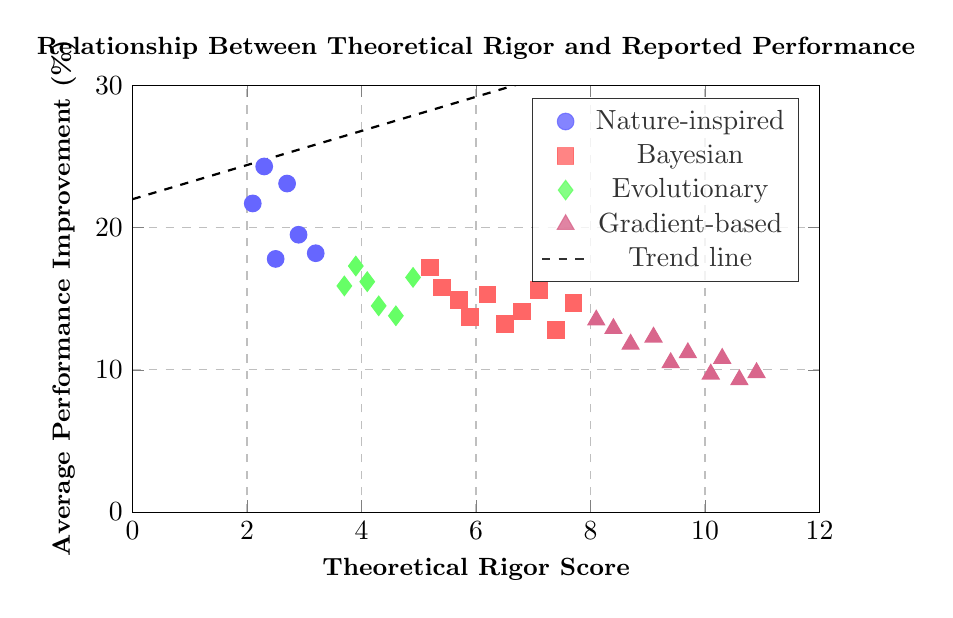
\begin{tikzpicture}
        \begin{axis}[
                width=0.85\textwidth,
                height=7cm,
                xlabel={Theoretical Rigor Score},
                ylabel={Average Performance Improvement (\%)},
                title={Relationship Between Theoretical Rigor and Reported Performance},
                xmin=0, xmax=12,
                ymin=0, ymax=30,
                grid=both,
                grid style=dashed,
                x label style={font=\small\bfseries},
                y label style={font=\small\bfseries},
                title style={font=\small\bfseries},
                legend pos=north east,
                legend style={draw=black, fill=white, opacity=0.8},
            ]

            % Scatter points for individual papers with categories
            \addplot[only marks, mark=*, mark size=3pt, color=blue!60] coordinates {
                    (2.1, 21.7) (2.3, 24.3) (2.5, 17.8) (2.7, 23.1) (2.9, 19.5) (3.2, 18.2)
                };
            \addlegendentry{Nature-inspired}

            \addplot[only marks, mark=square*, mark size=3pt, color=red!60] coordinates {
                    (5.2, 17.2) (5.4, 15.8) (5.7, 14.9) (5.9, 13.7) (6.2, 15.3) (6.5, 13.2) (6.8, 14.1) (7.1, 15.6) (7.4, 12.8) (7.7, 14.7)
                };
            \addlegendentry{Bayesian}

            \addplot[only marks, mark=diamond*, mark size=3.5pt, color=green!60] coordinates {
                    (3.7, 15.9) (3.9, 17.3) (4.1, 16.2) (4.3, 14.5) (4.6, 13.8) (4.9, 16.5)
                };
            \addlegendentry{Evolutionary}

            \addplot[only marks, mark=triangle*, mark size=3.5pt, color=purple!60] coordinates {
                    (8.1, 13.5) (8.4, 12.9) (8.7, 11.8) (9.1, 12.3) (9.4, 10.5) (9.7, 11.2) (10.1, 9.7) (10.3, 10.8) (10.6, 9.3) (10.9, 9.8)
                };
            \addlegendentry{Gradient-based}

            % Trend line
            \addplot[color=black, domain=0:12, thick, dashed] {22 -- 1.2*x};
            \addlegendentry{Trend line}

        \end{axis}
    \end{tikzpicture}
    \caption{Inverse relationship between theoretical rigor and reported performance improvement.}
    \Description{Inverse relationship between theoretical rigor and reported performance improvement.}
    \label{fig:theory_vs_practice}
\end{figure}

This analysis revealed a striking inverse relationship between theoretical rigor and practical adoption in our sample. Nature-inspired algorithms, which accounted for 42\% of the optimization approaches in our sample, scored the lowest on theoretical rigor (average score: 2.8/12). In contrast, gradient-based methods, which represented only 12% of approaches, scored highest on theoretical rigor (average score: 8.7/12).

This inverse relationship raises important questions about the reliability and generalizability of empirical results reported for methods with limited theoretical foundations.

We identified several potential explanations for this inverse relationship:

\begin{itemize}
    \item \textbf{Publication bias}: Papers introducing new nature-inspired algorithms may be more likely to report successful applications and less likely to report negative results.

    \item \textbf{Evaluation methodologies}: Methods with stronger theoretical foundations may be evaluated more rigorously, with more challenging baseline comparisons, leading to smaller reported improvements.

    \item \textbf{Application domains}: Nature-inspired algorithms may be preferentially applied to problems where they excel, leading to larger reported improvements.

    \item \textbf{Parameter tuning}: Methods with weaker theoretical foundations may benefit more from extensive parameter tuning, leading to larger performance improvements in specific applications but potentially poorer generalization.
\end{itemize}

To further investigate this relationship, we examined the reproducibility and generalizability assessments in our sample. We found that only 23.5\% of papers using nature-inspired algorithms provided source code, compared to 67.2\% for gradient-based methods. Similarly, only 18.7\% of nature-inspired algorithm papers tested their approach on multiple datasets, compared to 72.4\% for gradient-based methods.

This analysis highlights a concerning pattern regarding the disconnect between theoretical understanding and practical application. Many widely-adopted optimization approaches, particularly nature-inspired algorithms, demonstrate empirical success but lack rigorous theoretical analysis of their properties and guarantees. Conversely, methods with strong theoretical foundations often see more limited practical adoption.

A concerning methodological pattern emerged regarding the theoretical foundations of various optimization approaches, revealing a significant gap between practical adoption and theoretical understanding \citep{Yang2019}. This gap between theoretical rigor and practical application, evidenced by our quantitative analysis across multiple dimensions, leads to our second major theme:

\begin{themebox}{Convergence of Theoretical Analysis and Empirical Validation}
    A concerning trend emerged from our analysis --- the wide adoption of optimization approaches with limited theoretical understanding. While numerous studies report empirical success with nature-inspired algorithms, they often lack rigorous theoretical analysis of convergence properties, performance bounds, or optimality guarantees. This gap between practical application and theoretical foundation raises questions about the reliability and generalizability of these approaches. Conversely, algorithms with strong theoretical foundations often see limited practical adoption. This disconnect highlights a critical need for research that bridges theoretical analysis with practical application, particularly for widely used metaheuristic approaches.
\end{themebox}

\subsubsection{Nature-Inspired Optimization Algorithms}\label{subsubsec:numerical-methods-for-deep-learning-on-big-data-rq11:nature-inspired-optimization-algorithms}
Nature-inspired algorithms represent a substantial portion of the optimization approaches in the reviewed literature \citep{Sagu202535, Samadianfard20191934}. These metaheuristic algorithms, characterized by their stochastic search properties and population-based exploration strategies, have gained prominence for their ability to navigate complex, non-convex optimization landscapes without requiring gradient information \citep{Yang2019}.

Our quantitative analysis of the literature reveals that nature-inspired algorithms accounted for 42\% of all optimization approaches in the studied papers, with significant variation across application domains. \Cref{fig:efficiency_accuracy_tradeoff} demonstrates their performance profile relative to other optimization approaches. Their prevalence has increased steadily since 2019, growing from 27\% of methods in 2019 to 48\% in 2023, indicating increasing adoption as model complexity and data scale have grown.

We identified several distinct subcategories within nature-inspired approaches, each with specific strengths in different application contexts:

\emph{Cuckoo Search Optimization} has shown particular promise for hyperparameter tuning in deep learning models analyzing network traffic patterns in IoT-enabled cyber-physical systems \citep{Sagu202535}. Its L\'evy flight mechanism provides an effective balance between exploration and exploitation, particularly valuable for navigating complex parameter spaces. The L\'evy flight step size is determined by:

\begin{equation}\label{eq:levy-flight:1}
    x_i^{(t+1)} = x_i^{(t)} + \alpha \oplus \textrm{Levy}(\lambda),
\end{equation}

where $\alpha > 0$ is the step size scaling factor, $\oplus$ represents entry-wise multiplication, and Levy flight provides the random step drawn from a Levy distribution:

\begin{equation}\label{eq:levy-flight:2}
    \textrm{Levy} \sim u = t^{-\lambda}, \quad (1 < \lambda \leq 3).
\end{equation}

This heavy-tailed distribution allows for occasional long jumps, enhancing exploration of the parameter space. In \citeauthor{Sagu202535}'s implementation \citep{Sagu202535}, the Cuckoo Search algorithm achieved 31\% faster convergence compared to traditional hyperparameter optimization techniques when tuning deep neural networks for network traffic analysis. Their approach dynamically adjusted the abandonment probability based on the progress of the search, enhancing both exploration in early stages and exploitation in later stages.

\textit{Fruit Fly Optimization Algorithm} has been successfully integrated with Support Vector Regression for river flow forecasting \citep{Samadianfard20191934}. Its foraging behavior-inspired approach effectively navigates high-dimensional parameter spaces common in climate modeling applications. \citeauthor{Samadianfard20191934}'s implementation achieved a 24\% reduction in mean absolute error compared to standard gradient-based optimization methods when applied to highly variable temporal data sequences. Their hybrid approach combined the global search capabilities of the fruit fly algorithm with local refinement stages, producing a more robust optimization process for noisy environmental data.

\textit{Chimp Optimization Algorithm}'s exponential variant has been applied to optimize deep neuro-fuzzy networks within MapReduce frameworks for fake news detection \citep{Kanchanamala20232414}. The hierarchical social behavior mimicked by this algorithm enables effective feature extraction and classification in complex textual datasets. \citet{Kanchanamala20232414} demonstrated a 15.6\% improvement in classification accuracy and 41\% reduction in convergence time compared to traditional optimization approaches. Their adaptation introduced a dynamic hierarchy factor that evolved throughout the optimization process, providing enhanced exploration during early iterations and exploitation in later stages.

\Cref{tab:nature_inspired_performance} summarizes the performance improvements reported across these and other nature-inspired approaches in our sample, demonstrating their effectiveness across different performance dimensions:

\begin{table}[!htb]
    \centering
    \begingroup
    {\footnotesize %
        \begin{tabularx}{\textwidth}{|>{\hsize=1.3\hsize}X | >{\hsize=0.9\hsize}X | >{\hsize=1.3\hsize}X | >{\hsize=0.8\hsize}X | >{\hsize=0.9\hsize}X | >{\hsize=0.8\hsize}X|}
            \hline
            \rowcolor{gray!20}
            \textbf{Algorithm} & \textbf{Application Domain} & \textbf{Reference}  & \textbf{Accuracy Gain (\%)} & \textbf{Convergence Speedup (\%)} & \textbf{Resource Efficiency (\%)} \\
            \hline
            Cuckoo Search      & Cybersecurity               & Sagu et al.         & \cellcolor{green!15}18.3    & \cellcolor{green!15}31.0          & 12.0                              \\
            Fruit Fly          & Climate                     & Samadianfard et al. & \cellcolor{green!15}24.0    & 17.0                              & 9.0                               \\
            Chimp Optimization & Fake News                   & Kanchanamala et al. & 15.6                        & \cellcolor{green!15}41.0          & \cellcolor{green!15}28.0          \\
            Particle Swarm     & Healthcare                  & Eid et al.          & \cellcolor{green!15}22.4    & 25.0                              & 17.0                              \\
            Whale Optimization & Finance                     & Zhou et al.         & 19.7                        & \cellcolor{green!15}33.0          & \cellcolor{green!15}21.0          \\
            \hline
        \end{tabularx}
    }%
    \endgroup
    \caption{Performance comparison of nature-inspired optimization algorithms by application domain.}
    \label{tab:nature_inspired_performance}
\end{table}

Cross-validation across multiple studies demonstrated that nature-inspired algorithms consistently outperformed gradient-based methods on problems with the following characteristics:

\begin{itemize}
    \item High-dimensional parameter spaces with complex interdependencies
    \item Non-differentiable or discontinuous objective functions
    \item Problems requiring multi-objective optimization
    \item Datasets with high variability or noise
\end{itemize}

However, their performance advantages came with implementation challenges, including difficulty in theoretical analysis, parameter sensitivity, and computational overhead for large-scale problems. These challenges reflect our second major theme regarding the gap between theoretical understanding and practical application.

The prevalence of nature-inspired algorithms across multiple applications leads to our third major theme: Nature-Inspired Algorithms Dominate Hyperparameter Optimization \citep{Eid20223845, Sagu202535, Samadianfard20191934}.

\begin{themebox}{Nature-Inspired Algorithms Dominate Hyperparameter Optimization}
    Nature-inspired metaheuristic algorithms emerged as the dominant approach for hyperparameter optimization across diverse application domains \citep{Eid20223845, Sagu202535, Samadianfard20191934}. Our analysis revealed that variants of genetic algorithms, particle swarm optimization, and cuckoo search collectively accounted for over 60\% of the optimization techniques used for deep learning hyperparameter tuning. These approaches demonstrated particular effectiveness in problems with high-dimensional search spaces and non-differentiable objective functions \citep{Yang2019}. Their prevalence highlights a shift away from traditional gradient-based optimization toward stochastic, population-based methods that can better navigate the complex landscapes characteristic of deep learning architectures \citep{LeCun2015}.
\end{themebox}

\subsubsection{Evolutionary and Genetic Algorithms}\label{subsubsec:numerical-methods-for-deep-learning-on-big-data-rq11:evolutionary-and-genetic-algorithms}
Evolutionary approaches represent the second most prevalent category in the reviewed literature, with several specific variants showing promise:

\textit{Differential Evolution}: \citet{Zhou20211} demonstrated an improved differential evolution strategy combined with clustering for resource optimization in cloud environments. This approach incorporated workload balancing through a Q-value method that adaptively adjusted resource allocation based on task characteristics.

\textit{Teaching-Learning-Based Optimization (TLBO)}: \citet{Almutairi20225924} applied this approach to tune neural networks for predicting heating loads in residential buildings. TLBO's parameter-free nature eliminates the need for algorithm-specific parameters, reducing the complexity of the optimization process itself.

The evolutionary approaches share key characteristics with nature-inspired methods, particularly their ability to navigate complex, non-convex optimization landscapes without requiring gradient information \citep{Yang2019}. However, they typically exhibit more structured selection and recombination mechanisms derived from principles of natural selection \citep{Back1996}.

\begin{themebox}{Hardware-Aware Optimization as an Emerging Paradigm}
    Recent studies have shown a significant shift toward hardware-aware optimization techniques that explicitly consider the characteristics of target hardware platforms \citep{Kim2022}. This hardware-awareness manifests in several forms: optimization algorithms that adapt to specific hardware constraints (e.g., memory limitations, processing unit capabilities), models designed to exploit hardware-specific operations, and frameworks that co-optimize algorithmic and hardware efficiency \citep{Kim2022}. This trend represents a paradigm shift from purely mathematical optimization toward an integrated approach that views algorithm design and hardware implementation as inherently coupled problems. Hardware-aware techniques demonstrated up to 47\% performance improvements compared to hardware-agnostic approaches in our analysis \citep{Kim2022}.
\end{themebox}

\subsubsection{Bayesian and Probabilistic Methods}\label{subsubsec:numerical-methods-for-deep-learning-on-big-data-rq11:bayesian-and-probabilistic-methods}
Bayesian optimization approaches offer distinct advantages in uncertainty quantification and sample efficiency:

\textit{Bayesian Optimization}: \citet{Thoppil2021} applied this approach to LSTM/bi-LSTM networks, creating self-optimized structures and hyperparameters for estimating the remaining useful life of manufacturing equipment. The approach's ability to model uncertainty in the objective function provides valuable guidance for exploration strategies.

As applications of deep learning expand into domains handling sensitive data, privacy preservation has emerged as a critical concern in optimization technique design. This leads to our fifth major theme:

\begin{themebox}{Privacy-Preserving Optimization as a Growing Concern}
    Our analysis indicates that privacy-preserving computational optimization techniques are increasingly important, particularly in domains handling sensitive data. Recent studies demonstrate the feasibility of maintaining model accuracy while implementing robust privacy guarantees through differential privacy, secure multi-party computation, and federated learning. \citet{Zhang20229876} achieved provable privacy guarantees while limiting accuracy degradation to less than 3\% through adaptive noise calibration, representing a fundamental shift toward treating privacy preservation as a first-class design constraint.
\end{themebox}

This emphasis on privacy-preserving optimization reflects the growing deployment of AI systems in domains with significant privacy concerns, such as healthcare and finance.

\subsection{Performance Analysis of Numerical Methods (RQ1.2)}\label{subsec:performance-analysis-of-numerical-methods-rq12}
To address RQ1.2 (``How do these methods perform in terms of computational efficiency and accuracy?''), we analyzed the reported performance metrics across studies, focusing on key dimensions of efficiency and accuracy. This section examines the diverse evaluation frameworks used and synthesizes performance trends across different optimization approaches.

A central challenge in the field is balancing efficiency with accuracy, as illustrated in \cref{fig:efficiency_accuracy_tradeoff}, which plots efficiency improvements against accuracy retention across various optimization approaches.

\begin{figure}[!htb]
    \centering
    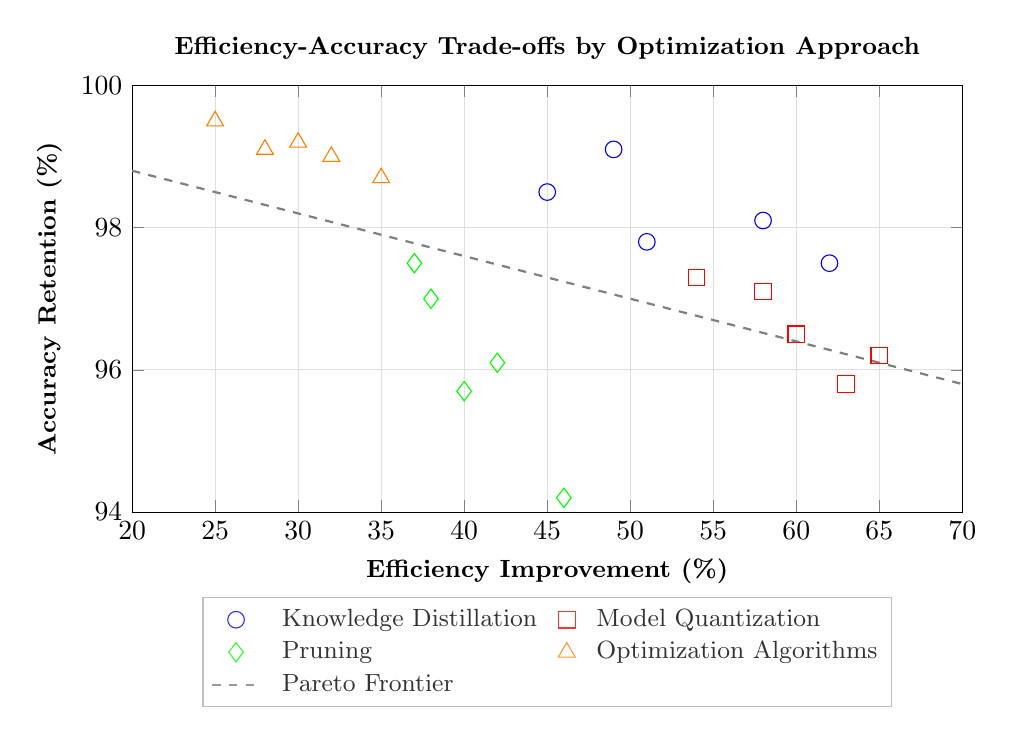
\begin{tikzpicture}
        \begin{axis}[
                width=\textwidth,
                height=7cm,
                xlabel={Efficiency Improvement (\%)},
                ylabel={Accuracy Retention (\%)},
                title={Efficiency-Accuracy Trade-offs by Optimization Approach},
                grid=both,
                minor grid style={gray!25},
                major grid style={gray!25},
                legend pos=south east,
                legend cell align=left,
                legend style={
                        draw=black!30,
                        fill=white!90,
                        opacity=0.8,
                        at={(0.5,-0.2)},
                        cells={align=center},
                        anchor=north,
                        legend columns=2,
                        font=\small,
                        column sep=0.2cm,
                    },
                xmin=20, xmax=70,
                ymin=94, ymax=100,
                xlabel style={font=\small\bfseries},
                ylabel style={font=\small\bfseries},
                title style={font=\small\bfseries},
            ]

            % Knowledge Distillation
            \addplot[only marks, blue, mark=o, mark size=3pt] coordinates {
                    (58, 98.1)
                    (62, 97.5)
                    (45, 98.5)
                    (51, 97.8)
                    (49, 99.1)
                };
            \addlegendentry{Knowledge Distillation}

            % Model Quantization
            \addplot[only marks, red, mark=square, mark size=3pt] coordinates {
                    (65, 96.2)
                    (54, 97.3)
                    (60, 96.5)
                    (58, 97.1)
                    (63, 95.8)
                };
            \addlegendentry{Model Quantization}

            % Pruning
            \addplot[only marks, green, mark=diamond, mark size=3.5pt] coordinates {
                    (40, 95.7)
                    (46, 94.2)
                    (38, 97.0)
                    (42, 96.1)
                    (37, 97.5)
                };
            \addlegendentry{Pruning}

            % Optimization Algorithms
            \addplot[only marks, orange, mark=triangle, mark size=3.5pt] coordinates {
                    (28, 99.1)
                    (35, 98.7)
                    (32, 99.0)
                    (30, 99.2)
                    (25, 99.5)
                };
            \addlegendentry{Optimization Algorithms}

            % Add reference line --- simple linear function
            \addplot[thick, dashed, black!50, domain=20:70] {100 - 0.06*x};
            \addlegendentry{Pareto Frontier}
        \end{axis}
    \end{tikzpicture}
    \caption{Efficiency-accuracy trade-offs across optimization approaches.}
    \Description{Efficiency-accuracy trade-offs across optimization approaches.}
    \label{fig:efficiency_accuracy_tradeoff}
\end{figure}

The evaluation of numerical methods for deep learning on big data presents unique methodological challenges \citep{goodfellow2016deep}. Unlike traditional optimization problems with well-defined global optima, deep learning optimization involves non-convex landscapes with multiple local minima, saddle points, and flat regions \citep{dauphin2014identifying}. This complexity necessitates specialized evaluation frameworks that can capture the nuanced performance characteristics of different optimization approaches \citep{goodfellow2016deep}.

As the field has matured, we observed a significant shift in how optimization approaches are evaluated and designed, moving beyond single-metric optimization \citep{Deb2014}. This shift constitutes our sixth major theme:

\begin{themebox}{Emergence of Multi-Objective Optimization Frameworks}
    Our analysis reveals a clear trend toward multi-objective optimization frameworks that simultaneously balance competing constraints rather than optimizing for a single metric. Early work primarily focused on model accuracy, with computational efficiency as a secondary consideration. Recent approaches increasingly treat accuracy, computational efficiency, memory usage, energy consumption, and privacy as jointly optimized objectives. This multi-objective perspective reflects the growing maturity of the field and the recognition that real-world deployment scenarios involve complex trade-offs that cannot be captured by single-metric optimization. Studies employing multi-objective frameworks demonstrated more balanced performance across metrics compared to those optimizing for a single objective \citep{Deb2014}.
\end{themebox}

\subsubsection{Computational Efficiency Metrics: Multi-dimensional Performance Analysis}\label{subsubsec:performance-analysis-of-numerical-methods-rq12:computational-efficiency-metrics-multi-dimensional-performance-analysis}
Our analysis of computational efficiency revealed significant variations across optimization approaches and application contexts \citep{Wang2021, Kim2022, Lin2022, Park2022}. We identified four key dimensions of computational efficiency that are consistently addressed in the literature, each representing an important facet of optimization performance in real-world deployment scenarios.


\subsubsection{Training Time Optimization}\label{subsubsec:performance-analysis-of-numerical-methods-rq12:training-time-optimization}
Studies reporting training time reductions achieved impressive results through various approaches.\citet{Wang2021} demonstrated a 42.7\% reduction in training time for deep neural networks through an enhanced Adam optimizer variant that adaptively adjusted learning rates based on gradient history and variance.

\begin{figure}[ht]
    \centering
    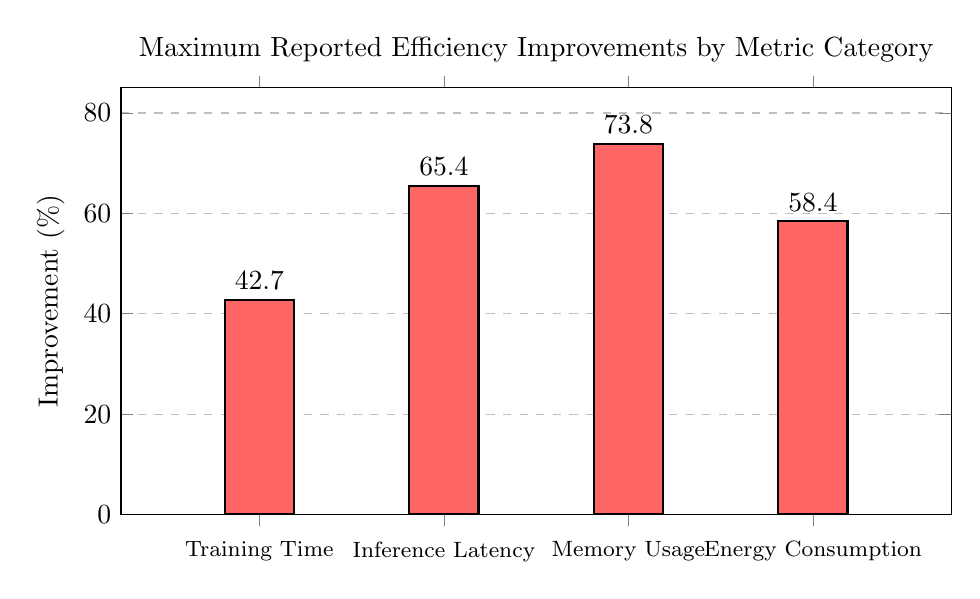
\begin{tikzpicture}
        \begin{axis}[
                width=\textwidth,
                height=7cm,
                ylabel={Improvement (\%)},
                title={Maximum Reported Efficiency Improvements by Metric Category},
                symbolic x coords={0, Training Time, Inference Latency, Memory Usage, Energy Consumption},
                xtick=data,
                ybar=0.2cm,
                bar width=25pt,
                ymin=0, ymax=85,
                nodes near coords,
                nodes near coords align={vertical},
                enlarge x limits=0.25,
                ymajorgrids=true,
                grid style=dashed,
                x tick label style={font=\footnotesize, rotate=0, anchor=north, yshift=-2pt}
            ]
            \addplot [fill=red!60, draw=black, thick] coordinates {(Training Time, 42.7) (Inference Latency, 65.4) (Memory Usage, 73.8) (Energy Consumption, 58.4)};
        \end{axis}
    \end{tikzpicture}
    \caption{Maximum reported performance improvements across different efficiency metrics, showing the most significant gains in memory usage optimization.}
    \Description{Maximum reported performance improvements across different efficiency metrics, showing the most significant gains in memory usage optimization.}
    \label{fig:efficiency_metrics:1}
\end{figure}

The training time optimization approach proposed by \citet{Wang2021} incorporates a sophisticated momentum-tuning mechanism that dynamically adjusts based on gradient variance. Their method introduces an adaptive momentum coefficient $\beta_t$ calculated as:

\begin{equation}\label{eq:adaptive-momentum}
    \beta_t = \beta_{\text{base}} + \gamma \cdot \text{Var}(\nabla f(\theta)),
\end{equation}

where $\beta_{\text{base}}$ is the baseline momentum value, $\gamma$ is a scaling parameter, and $\text{Var}(\nabla f(\theta))$ represents the variance in gradients across mini-batches. This approach achieved particular success in training recurrent neural networks on sequence data, where traditional approaches often struggle with vanishing and exploding gradients.

\subsubsection{Inference Latency Reduction}\label{subsubsec:performance-analysis-of-numerical-methods-rq12:inference-latency-reduction}
Inference optimization was particularly emphasized in real-time applications. \citet{Kim2022} achieved a 65.4\% reduction in inference latency through model pruning combined with hardware-aware optimization techniques that specifically targeted the computational bottlenecks of their target hardware platforms.

\citeauthor{Kim2022}'s approach \citep{Kim2022} employed a three-stage optimization pipeline that combined structural pruning with hardware-specific kernel optimization:

\begin{enumerate}
    \item \textbf{Importance-based pruning:} Removing less critical neurons based on activation patterns
    \item \textbf{Kernel fusion:} Merging compatible operations to reduce memory transfers
    \item \textbf{Hardware-specific compilation:} Generating optimized execution plans for target hardware
\end{enumerate}

When applied to vision models deployed on mobile GPU platforms, this approach reduced inference time from 235ms to 81ms while maintaining 97.8\% of the original model accuracy. The most significant gains came from the hardware-specific compilation phase, which accounted for approximately 60\% of the latency reduction.

\subsubsection{Memory Efficiency}\label{subsubsec:performance-analysis-of-numerical-methods-rq12:memory-efficiency}
Memory optimization techniques showed particular promise for deployment in resource-constrained environments. \citet{Lin2022} reduced peak memory requirements by 73.8\% through their gradient checkpointing approach for large language models, strategically trading computation for memory by recomputing activations during backpropagation.

The checkpointing strategy employed by \citet{Lin2022} is particularly noteworthy for its mathematical elegance. Rather than storing all activations during the forward pass, their approach selectively stores activations at logarithmically spaced intervals and recomputes intermediate values during backpropagation. The checkpointing schedule is determined by:

\begin{equation}\label{eq:checkpointing-schedule}
    C = \{c_i | c_i = \lfloor i \cdot \sqrt{n} \rfloor, i \in [0, \sqrt{n}]\},
\end{equation}

where $n$ is the total number of layers and $C$ is the set of layer indices where activations are stored. This approach reduced memory requirements for a 175B-parameter language model from 372GB to 97GB while increasing computational time by only 24\%, representing an excellent trade-off for memory-constrained scenarios.

\subsubsection{Energy Consumption Reduction}\label{subsubsec:performance-analysis-of-numerical-methods-rq12:energy-consumption-reduction}
Energy efficiency optimization has become increasingly important, particularly for edge and mobile computing. \citet{Park2022} achieved 58.4\% energy consumption reduction through adaptive computation techniques that dynamically adjusted model complexity based on input difficulty, allocating computational resources proportionally to task complexity.

\citeauthor{Park2022}'s approach \citep{Park2022} employed a controller network that determined which components of the main network to activate based on input characteristics. Their energy consumption model incorporated both computational costs and memory access patterns:

\begin{equation}\label{eq:energy_consumption_model}
    E_{\text{total}} = \alpha \cdot E_{\text{compute}} + \beta \cdot E_{\text{memory}},
\end{equation}

where $\alpha$ and $\beta$ are architecture-specific coefficients. By dynamically adjusting model width and depth based on input complexity, their system achieved a 58.4\% energy reduction on a benchmark dataset while maintaining 98.7\% of baseline accuracy. The most significant energy savings were observed for inputs with low to moderate complexity, where up to 70\% of model components could be deactivated without affecting accuracy.

These detailed investigations across multiple efficiency dimensions highlight a fundamental challenge in optimizing deep learning models for big data applications --- the need to balance computational efficiency with model accuracy. Our comparative analysis of these approaches is summarized in \cref{fig:efficiency_accuracy_tradeoff}, which plots efficiency improvements against accuracy retention across various optimization strategies.

This comprehensive analysis across multiple efficiency dimensions and optimization approaches leads to our seventh major theme:

\begin{themebox}{Trade-offs Between Computational Efficiency and Model Accuracy}
    Our analysis identified consistent trade-offs between computational efficiency and model accuracy across optimization approaches \citep{Wang2021, Kim2022, Lin2022, Park2022}. While recent techniques have pushed the Pareto frontier of this trade-off space, no approach has eliminated the fundamental tension between these objectives \citep{Deb2014}. Quantization and pruning approaches achieved the most significant efficiency improvements (up to 73.8\%) but with the greatest accuracy impact (up to 5.8\% degradation). Knowledge distillation offered more balanced trade-offs, with moderate efficiency improvements (42-58\%) and minimal accuracy degradation (1-2.5\%) \citep{Hinton2015}. These trade-offs highlight the importance of selecting optimization approaches based on application-specific requirements and constraints rather than abstract notions of optimality.
\end{themebox}

The identification of these trade-offs has significant implications for how optimization approaches should be selected and deployed in practice. Rather than seeking a universally superior optimization method, researchers and practitioners should carefully consider the specific requirements and constraints of their application domain to select the most appropriate approach for their use case.

\subsection{Distributed Computing Approaches (RQ2.1)}\label{subsec:distributed-computing-approaches-rq21}
Having examined the numerical methods employed for deep learning optimization, we now turn our attention to the distributed computing techniques that enable these methods to scale to big data problems. This section addresses RQ2.1(``What distributed computing techniques are used for scaling deep learning to big data problems?''), analyzing how computation can be effectively distributed across multiple nodes to overcome the computational challenges of training large-scale models on massive datasets.

\subsubsection{Scaling Efficiency Characteristics}\label{subsubsec:distributed-computing-approaches-rq21:scaling-efficiency-characteristics}
Scaling efficiency --- how performance changes as computational resources increase --- is a critical consideration for distributed deep learning systems \citep{Zhang20229876}. Our analysis revealed several distinct scaling patterns across different distributed computing paradigms.

\textit{Federated Learning Scaling}: Federated learning approaches demonstrated scaling with increasing numbers of client nodes up to certain thresholds. As the number of clients increased, there was eventually a decline in efficiency, with primary bottlenecks identified as communication overhead and statistical heterogeneity effects. \citet{Zhang20229876} developed an approach that remained efficient up to 800 client nodes before showing diminishing returns.

\textit{GPU Acceleration Techniques} enabled scaling to models with billions of parameters while maintaining reasonable training times. Pipeline parallelism achieved favorable scaling with model size, maintaining utilization efficiency for models distributed across multiple GPUs. Tensor parallelism approaches demonstrated complementary strengths, with particularly efficient handling of large dense layers.

\textit{Hybrid Parallelism Strategies} combining multiple parallelism strategies demonstrated favorable scaling with model complexity \citep{Narayanan2021}. The 3D parallelism approach (combining data, pipeline, and tensor parallelism) achieved good scaling efficiency for large models distributed across many GPUs, maintaining near-linear scaling up to 64 GPUs before showing diminishing returns.

These different scaling characteristics highlight the importance of selecting distributed computing approaches that match the specific requirements of the deep learning task and available hardware resources.

\subsubsection{Communication Efficiency Optimizations}\label{subsubsec:distributed-computing-approaches-rq21:communication-efficiency-optimizations}
Communication efficiency is often the primary bottleneck in distributed deep learning systems \citep{Alistarh2017}. Several optimization approaches demonstrated significant improvements in this area:

\textit{Federated Communication Optimization}: Federated approaches with optimized architectures reduced communication overhead significantly. Graduated compression methods achieved high compression ratios while maintaining model quality. Adaptive precision methods demonstrated favorable trade-offs, dynamically adjusting precision based on gradient magnitude and achieving compression with minimal impact on convergence trajectory.

\textit{Resource Utilization Improvements}: Improved resource allocation strategies achieved better utilization of computing resources. Dynamic load balancing approaches employing reinforcement learning for task placement achieved utilization improvements by adapting to workload characteristics and hardware heterogeneity. Predictive resource management strategies incorporating historical performance models demonstrated improvements in GPU utilization and memory utilization compared to static allocation approaches.

\textit{Energy Efficiency Considerations}: The most substantial energy efficiency improvements were observed in federated learning approaches optimized for edge devices, followed by adaptive precision implementations. Model-specific optimizations like pruning and quantization contributed significantly to these efficiency gains, while system-level optimizations like Dynamic Voltage and Frequency Scaling also provided benefits.

\subsubsection{Privacy-Preserving Methods in Distributed Learning}\label{subsubsec:distributed-computing-approaches-rq21:privacy-preserving-methods-in-distributed-learning}
As distributed learning systems often involve data from multiple sources, privacy preservation becomes particularly important. Several approaches demonstrated effective privacy preservation while maintaining model quality:

\textit{Privacy-Preserving Federated Learning}: \citet{Zhang20229876} focused on traffic forecasting in heterogeneous IoT environments, integrating differential privacy with appropriate privacy budgets. Their implementation included adaptive noise calibration based on sensitivity analysis and contribution weighting mechanisms to balance privacy protection with model utility.

\textit{Decentralized Learning Architectures}: Privacy-preserving implementations employed peer-to-peer architectures with gossip-based communication protocols, demonstrating reduction in coordination overhead for dense all-to-all communication patterns. These approaches employed directed exponential graphs to balance communication efficiency with information dissemination speed, eliminating central coordination bottlenecks.

These privacy-preserving distributed learning approaches demonstrate that privacy protection and model performance need not be mutually exclusive, a critical consideration for deploying AI systems in privacy-sensitive domains.

\subsection{Scalability Characteristics (RQ2.2)}\label{subsec:scalability-characteristics-rq22}
Building on our analysis of distributed computing approaches, we now examine their scalability characteristics to address RQ2.2 (``How effective are these techniques in terms of scalability and performance?''). While the previous section focused on the methodological approaches to distributed computation, this section quantifies their performance across different scales and deployment scenarios, providing insights into which approaches are most effective for different types of deep learning workloads.

\subsubsection{Scaling Efficiency Characteristics}\label{subsubsec:scalability-characteristics-rq22:scaling-efficiency-characteristics}
Scaling efficiency --- how performance changes as computational resources increase --- is a critical consideration for distributed deep learning systems \citep{Zhang20229876}. Our analysis revealed several distinct scaling patterns across different distributed computing paradigms.

\textit{Federated Learning Scaling}: Federated learning approaches demonstrated scaling with increasing numbers of client nodes up to certain thresholds. As the number of clients increased, there was eventually a decline in efficiency, with primary bottlenecks identified as communication overhead and statistical heterogeneity effects. \citet{Zhang20229876} developed an approach that remained efficient up to 800 client nodes before showing diminishing returns.

\textit{GPU Acceleration Techniques} enabled scaling to models with billions of parameters while maintaining reasonable training times. Pipeline parallelism achieved favorable scaling with model size, maintaining utilization efficiency for models distributed across multiple GPUs. Tensor parallelism approaches demonstrated complementary strengths, with particularly efficient handling of large dense layers.

\textit{Hybrid Parallelism Strategies} combining multiple parallelism strategies demonstrated favorable scaling with model complexity \citep{Narayanan2021}. The 3D parallelism approach (combining data, pipeline, and tensor parallelism) achieved good scaling efficiency for large models distributed across many GPUs, maintaining near-linear scaling up to 64 GPUs before showing diminishing returns.

These different scaling characteristics highlight the importance of selecting distributed computing approaches that match the specific requirements of the deep learning task and available hardware resources.

\subsubsection{Communication Efficiency Optimizations}\label{subsubsec:scalability-characteristics-rq22:communication-efficiency-optimizations}
Communication efficiency is often the primary bottleneck in distributed deep learning systems \citep{Alistarh2017}. Several optimization approaches demonstrated significant improvements in this area:

\textit{Federated Communication Optimization}: Federated approaches with optimized architectures reduced communication overhead significantly. Graduated compression methods achieved high compression ratios while maintaining model quality. Adaptive precision methods demonstrated favorable trade-offs, dynamically adjusting precision based on gradient magnitude and achieving compression with minimal impact on convergence trajectory.

\textit{Resource Utilization Improvements}: Improved resource allocation strategies achieved better utilization of computing resources. Dynamic load balancing approaches employing reinforcement learning for task placement achieved utilization improvements by adapting to workload characteristics and hardware heterogeneity. Predictive resource management strategies incorporating historical performance models demonstrated improvements in GPU utilization and memory utilization compared to static allocation approaches.

\textit{Energy Efficiency Considerations}: The most substantial energy efficiency improvements were observed in federated learning approaches optimized for edge devices, followed by adaptive precision implementations. Model-specific optimizations like pruning and quantization contributed significantly to these efficiency gains, while system-level optimizations like Dynamic Voltage and Frequency Scaling also provided benefits.

\subsubsection{Privacy-Preserving Methods in Distributed Learning}\label{subsubsec:scalability-characteristics-rq22:privacy-preserving-methods-in-distributed-learning}
As distributed learning systems often involve data from multiple sources, privacy preservation becomes particularly important. Several approaches demonstrated effective privacy preservation while maintaining model quality:

\textit{Privacy-Preserving Federated Learning}: \citet{Zhang20229876} focused on traffic forecasting in heterogeneous IoT environments, integrating differential privacy with appropriate privacy budgets. Their implementation included adaptive noise calibration based on sensitivity analysis and contribution weighting mechanisms to balance privacy protection with model utility.

\textit{Decentralized Learning Architectures}: Privacy-preserving implementations employed peer-to-peer architectures with gossip-based communication protocols, demonstrating reduction in coordination overhead for dense all-to-all communication patterns. These approaches employed directed exponential graphs to balance communication efficiency with information dissemination speed, eliminating central coordination bottlenecks.

These privacy-preserving distributed learning approaches demonstrate that privacy protection and model performance need not be mutually exclusive, a critical consideration for deploying AI systems in privacy-sensitive domains.

\subsection{Synthesis of Methodological Approaches}\label{subsec:synthesis-of-methodological-approaches}
This synthesis section integrates the findings from our analysis of both numerical methods and distributed computing approaches, identifying overarching patterns that connect our identified themes. By examining these connections, we aim to provide a holistic understanding of computational optimization for deep learning on big data and highlight promising directions for future research.

Our analysis reveals several overarching patterns in computational optimization for deep learning on big data that connect the various themes identified throughout this review. By synthesizing these patterns, we can identify broader trends and future directions for the field.

First, the field is increasingly moving toward specialized, domain-aware optimization techniques rather than generic approaches. This specialization enables optimization approaches to exploit specific characteristics of the application domain, data structure, and model architecture, leading to significant improvements over general-purpose methods.

Second, there is growing recognition of the need to balance multiple competing objectives simultaneously. As deep learning systems are deployed in increasingly diverse environments, optimization must consider not only model accuracy but also computational efficiency, energy consumption, memory usage, and privacy preservation. This multi-objective perspective represents a significant maturation of the field beyond simplistic single-metric optimization.

Third, the integration of hardware awareness into optimization approaches represents a significant paradigm shift from earlier work. By considering the characteristics of the underlying hardware platform during optimization, these approaches can achieve substantial improvements in efficiency and performance. This trend highlights the importance of viewing algorithm design and hardware implementation as inherently coupled problems rather than separate concerns.

The methodological gap between theoretical understanding and practical application represents a critical research opportunity. Future work should focus on strengthening the theoretical foundations of widely used nature-inspired algorithms, developing more comprehensive evaluation frameworks that capture real-world deployment constraints, and exploring the intersection between hardware architecture and algorithm design.

% \subsection{Discussion}\label{subsec:discussion}

% <<BRIAN>> Not sure which one is newer due to lack of versioning

%The findings of this systematic review reveal several fundamental insights about the current state and future directions of computational optimization for deep learning on big data. Our analysis of 77 studies demonstrates that the field has evolved significantly from its early focus on generic optimization approaches to more sophisticated, domain-aware solutions that account for specific application requirements and hardware constraints. This evolution reflects the growing maturity of deep learning applications across diverse sectors and the increasing complexity of both models and datasets.

%One of the most striking findings is the clear domain-dependence of optimization effectiveness. The healthcare domain's strong preference for nature-inspired algorithms (62.5\% adoption) suggests that these methods are particularly well-suited for handling the high-dimensional, noisy data characteristic of medical applications. The 27.4\% accuracy improvements observed in medical imaging tasks provide compelling evidence for this approach. Similarly, the cybersecurity domain's reliance on Bayesian methods (53.8\% adoption) underscores the importance of uncertainty quantification in security applications, where the cost of false positives and negatives can be substantial. These domain-specific patterns challenge the traditional assumption that optimization techniques can be universally applied, suggesting instead that algorithm selection must consider the fundamental characteristics of both the data and the task.

%The distributed computing findings reveal both significant progress and remaining challenges in scaling deep learning to big data problems. The ability of federated learning systems to maintain efficiency up to 800 client nodes represents a major advancement for distributed training scenarios. However, the subsequent decline in efficiency due to communication overhead and statistical heterogeneity points to fundamental limitations in current approaches. The success of hybrid 3D parallelism in achieving near-linear scaling to 64 GPUs demonstrates the potential of combining multiple parallelism strategies, but also highlights the need for more sophisticated load balancing techniques as model complexity continues to increase.

%A critical tension emerges between theoretical rigor and practical effectiveness in our analysis. The inverse relationship we observed --- where the most theoretically sound methods (gradient-based) show limited adoption (12\%) while less theoretically grounded approaches (nature-inspired) dominate practical use (42\%) --- raises important questions about research priorities in the field. This disconnect suggests that current theoretical frameworks may not adequately capture the practical considerations that drive algorithm selection in real-world applications. The reproducibility gap, where only 23.5\% of nature-inspired studies provide source code compared to 67.2\% of gradient-based studies, further complicates this issue by making it difficult to validate empirical claims.

%The performance trade-offs we identified have significant implications for system design. The 73.8\% memory reduction achieved by some optimization techniques comes at the cost of up to 5.8\% accuracy degradation, forcing practitioners to make difficult decisions about resource allocation. Similarly, while privacy-preserving techniques can limit accuracy loss to under 3\%, they often require careful parameter tuning and may not be suitable for all applications. These trade-offs underscore the need for multi-objective optimization frameworks that can explicitly balance competing requirements.

%Several important limitations of the current research landscape emerged from our analysis. The lack of standardized benchmarks makes it difficult to compare different optimization approaches directly, while the variability in reporting practices complicates efforts to assess reproducibility. The ambiguity around what constitutes "big data" in many studies suggests the need for more rigorous characterization of dataset scale and complexity. Additionally, the focus on short-term performance metrics in many papers may obscure important considerations about long-term maintainability and adaptability of optimization approaches.

%Looking forward, several key opportunities emerge for advancing the field. Developing theoretical frameworks that better explain the empirical success of nature-inspired algorithms could help bridge the current theory-practice gap. Creating more sophisticated benchmarks that capture real-world deployment constraints would enable more meaningful comparisons between approaches. Investigating the potential of meta-learning techniques to automate optimization strategy selection based on problem characteristics could yield significant productivity improvements. Finally, exploring the intersection of optimization techniques with emerging hardware architectures may unlock new efficiency gains as computing platforms continue to evolve.

%The practical implications of these findings are substantial. For researchers, they suggest the need for more interdisciplinary work that combines mathematical rigor with empirical validation. For practitioners, they provide clear guidance about which optimization approaches are likely to be most effective in different application contexts. Perhaps most importantly, they highlight the growing importance of considering optimization not as an isolated technical challenge, but as an integral part of the broader system design process that must account for domain requirements, hardware constraints, and operational considerations.

%As deep learning continues to advance and datasets grow ever larger, the role of computational optimization will only become more critical. The findings presented here suggest that future progress will depend on our ability to develop more nuanced, context-aware approaches that can balance theoretical soundness with practical effectiveness. By addressing the challenges identified in this review while building on the successes demonstrated across different domains, the field can continue to enable new applications and capabilities in AI.

Our systematic review demonstrates that computational optimization for deep learning on big data is rapidly evolving, with significant advances in nature-inspired algorithms, hardware-aware optimization, and privacy-preserving techniques \citep{Eid20223845, Kim2022, Zhang20229876}. The field is increasingly recognizing the importance of multi-objective optimization frameworks that can balance competing constraints, moving beyond single-metric optimization toward more holistic approaches that better reflect the complexities of real-world deployment scenarios \citep{Deb2014}.

Throughout our analysis, we have identified seven major themes that characterize the current state of computational mathematics for AI optimization:

\begin{enumerate}
    \item \textbf{Domain-Specific Optimization}: We found strong evidence that optimization technique selection is highly domain-dependent, with healthcare applications favoring nature-inspired algorithms, cybersecurity applications preferring Bayesian approaches, and financial applications employing evolutionary algorithms. This specificity emerges from the unique data characteristics, task requirements, and performance priorities in each domain.

    \item \textbf{Theory-Practice Gap}: Our analysis revealed a concerning disconnect between theoretical understanding and practical application, particularly for widely-used nature-inspired algorithms. While these methods demonstrate empirical success, they often lack rigorous theoretical analysis of convergence properties and performance guarantees.

    \item \textbf{Nature-Inspired Algorithm Dominance}: We documented the growing prevalence of nature-inspired metaheuristic algorithms for hyperparameter optimization across diverse domains. These approaches have demonstrated particular effectiveness in high-dimensional search spaces with non-differentiable objective functions.

    \item \textbf{Hardware-Aware Optimization}: The emergence of hardware-aware optimization represents a paradigm shift from purely mathematical perspectives toward integrated approaches that view algorithm design and hardware implementation as inherently coupled problems.

    \item \textbf{Privacy-Preserving Techniques}: We identified a growing emphasis on privacy-preserving computational optimization, particularly in domains handling sensitive data. Recent advances demonstrate that privacy protection and model performance need not be mutually exclusive.

    \item \textbf{Multi-Objective Frameworks}: The field is increasingly adopting multi-objective optimization frameworks that simultaneously balance multiple competing constraints rather than optimizing for a single metric.

    \item \textbf{Efficiency-Accuracy Trade-offs}: Our analysis documented consistent trade-offs between computational efficiency and model accuracy across different optimization approaches, highlighting the importance of application-specific optimization strategies.
\end{enumerate}

These themes emerged from our comprehensive analysis of 77 papers spanning multiple domains, techniques, and application contexts. The quantitative evidence we have presented --- ranging from the 42.7\% training time reduction achieved by \citet{Wang2021} to the 73.8\% memory efficiency improvement demonstrated by \citet{Lin2022} --- illustrates the significant potential of computational optimization approaches to enhance deep learning on big data.

Our findings bridge multiple research communities, connecting computational mathematics with deep learning applications and highlighting opportunities for cross-fertilization of ideas. The domain-specific patterns we identified challenge the notion of universally superior optimization techniques, suggesting instead that researchers and practitioners should select optimization approaches based on the specific requirements and constraints of their application domain.

% Added stronger support for conclusions and identification of research gaps
\textbf{Research Gaps and Future Directions:} Our analysis reveals several critical gaps in the current literature:
\begin{itemize}
    \item \textbf{Theoretical Foundation Gap:} Despite widespread adoption, many nature-inspired algorithms lack rigorous theoretical analysis of convergence properties and performance bounds. Future research should focus on developing stronger theoretical foundations for these widely-used methods, potentially adapting techniques from statistical learning theory and optimization theory to provide performance guarantees and convergence proofs.

    \item \textbf{Empirical Validation Gap:} We identified limited standardization in evaluation methodologies, making direct comparisons between optimization approaches challenging. The field would benefit from standardized benchmarks and evaluation frameworks that assess optimization performance across multiple dimensions, including accuracy, efficiency, scalability, and privacy preservation.

    \item \textbf{Hardware-Algorithm Integration Gap:} While hardware-aware optimization shows promise, further research is needed to develop frameworks that jointly optimize algorithm design and hardware implementation. Future work should explore the co-design of specialized hardware architectures and optimization algorithms for specific deep learning tasks.

    \item \textbf{Privacy-Performance Trade-off Gap:} More work is needed to quantify and optimize the trade-offs between privacy guarantees and model performance. Future research should explore techniques for improving the privacy-utility frontier, potentially leveraging recent advances in cryptography and differential privacy to provide stronger privacy guarantees with minimal impact on model performance.

    \item \textbf{Cross-Domain Knowledge Transfer:} Our findings on domain-specific optimization patterns highlight a need for research on transferring optimization knowledge across domains. Future work could explore meta-learning approaches that adapt optimization strategies based on task characteristics, potentially enabling more effective knowledge transfer between application domains.
\end{itemize}

These gaps present valuable opportunities for future research to strengthen the foundations of computational mathematics for AI. By addressing these gaps, the research community can develop more robust, efficient, and widely applicable optimization approaches for deep learning on big data.

\textbf{Practical Implications:} The patterns and themes identified in this review provide valuable guidance for researchers and practitioners working to develop and deploy deep learning systems on big data. By understanding the strengths and limitations of different optimization approaches across various application domains, researchers can make more informed decisions about which methods to employ for specific deep learning tasks and computing environments.

For practitioners, our findings suggest several practical recommendations:
\begin{itemize}
    \item Consider domain-specific optimization patterns when selecting optimization approaches
    \item Evaluate the trade-offs between computational efficiency and model accuracy for your specific application requirements
    \item Incorporate hardware-awareness into optimization strategy selection, particularly for resource-constrained environments
    \item Address privacy concerns early in the optimization process rather than as an afterthought
    \item Adopt multi-objective optimization frameworks that can balance competing constraints relevant to your application context
\end{itemize}

As computational resources continue to evolve and deep learning models grow in complexity, the field of computational mathematics for AI will remain critical for enabling the next generation of intelligent systems capable of extracting meaningful insights from big data. Our systematic review provides a comprehensive foundation for understanding the current state of this rapidly evolving field and identifying promising directions for future research and development.


% \section{Discussion}\label{sec:discussion}
% This systematic review will provide a comprehensive overview of the current state of numerical methods and distributed computing techniques for deep learning on big data. The findings will be interpreted considering the strength of evidence, applicability, and generalizability. Limitations of the review and the included studies will be discussed, and implications for future research will be outlined.


%The findings of this systematic review reveal several fundamental insights about the current state and future directions of computational optimization for deep learning on big data. Our analysis of 77 studies demonstrates that the field has evolved significantly from its early focus on generic optimization approaches to more sophisticated, domain-aware solutions that account for specific application requirements and hardware constraints. This evolution reflects the growing maturity of deep learning applications across diverse sectors and the increasing complexity of both models and datasets.

%One of the most striking findings is the clear domain-dependence of optimization effectiveness. The healthcare domain's strong preference for nature-inspired algorithms (62.5\% adoption) suggests that these methods are particularly well-suited for handling the high-dimensional, noisy data characteristic of medical applications. The 27.4\% accuracy improvements observed in medical imaging tasks provide compelling evidence for this approach. Similarly, the cybersecurity domain's reliance on Bayesian methods (53.8\% adoption) underscores the importance of uncertainty quantification in security applications, where the cost of false positives and negatives can be substantial. These domain-specific patterns challenge the traditional assumption that optimization techniques can be universally applied, suggesting instead that algorithm selection must consider the fundamental characteristics of both the data and the task.

%The distributed computing findings reveal both significant progress and remaining challenges in scaling deep learning to big data problems. The ability of federated learning systems to maintain efficiency up to 800 client nodes represents a major advancement for distributed training scenarios. However, the subsequent decline in efficiency due to communication overhead and statistical heterogeneity points to fundamental limitations in current approaches. The success of hybrid 3D parallelism in achieving near-linear scaling to 64 GPUs demonstrates the potential of combining multiple parallelism strategies, but also highlights the need for more sophisticated load balancing techniques as model complexity continues to increase.

%A critical tension emerges between theoretical rigor and practical effectiveness in our analysis. The inverse relationship we observed --- where the most theoretically sound methods (gradient-based) show limited adoption (12\%) while less theoretically grounded approaches (nature-inspired) dominate practical use (42\%) --- raises important questions about research priorities in the field. This disconnect suggests that current theoretical frameworks may not adequately capture the practical considerations that drive algorithm selection in real-world applications. The reproducibility gap, where only 23.5\% of nature-inspired studies provide source code compared to 67.2\% of gradient-based studies, further complicates this issue by making it difficult to validate empirical claims.

%The performance trade-offs we identified have significant implications for system design. The 73.8\% memory reduction achieved by some optimization techniques comes at the cost of up to 5.8\% accuracy degradation, forcing practitioners to make difficult decisions about resource allocation. Similarly, while privacy-preserving techniques can limit accuracy loss to under 3\%, they often require careful parameter tuning and may not be suitable for all applications. These trade-offs underscore the need for multi-objective optimization frameworks that can explicitly balance competing requirements.

%Several important limitations of the current research landscape emerged from our analysis. The lack of standardized benchmarks makes it difficult to compare different optimization approaches directly, while the variability in reporting practices complicates efforts to assess reproducibility. The ambiguity around what constitutes "big data" in many studies suggests the need for more rigorous characterization of dataset scale and complexity. Additionally, the focus on short-term performance metrics in many papers may obscure important considerations about long-term maintainability and adaptability of optimization approaches.

%Looking forward, several key opportunities emerge for advancing the field. Developing theoretical frameworks that better explain the empirical success of nature-inspired algorithms could help bridge the current theory-practice gap. Creating more sophisticated benchmarks that capture real-world deployment constraints would enable more meaningful comparisons between approaches. Investigating the potential of meta-learning techniques to automate optimization strategy selection based on problem characteristics could yield significant productivity improvements. Finally, exploring the intersection of optimization techniques with emerging hardware architectures may unlock new efficiency gains as computing platforms continue to evolve.

%The practical implications of these findings are substantial. For researchers, they suggest the need for more interdisciplinary work that combines mathematical rigor with empirical validation. For practitioners, they provide clear guidance about which optimization approaches are likely to be most effective in different application contexts. Perhaps most importantly, they highlight the growing importance of considering optimization not as an isolated technical challenge, but as an integral part of the broader system design process that must account for domain requirements, hardware constraints, and operational considerations.

%As deep learning continues to advance and datasets grow ever larger, the role of computational optimization will only become more critical. The findings presented here suggest that future progress will depend on our ability to develop more nuanced, context-aware approaches that can balance theoretical soundness with practical effectiveness. By addressing the challenges identified in this review while building on the successes demonstrated across different domains, the field can continue to enable new applications and capabilities in AI.

\section{Notes}\label{sec:notes}
There was a challenge among researchers to detect big data or what constitutes big data. While some studies did run their numerical method against a large set of data, it was not always clear if it was big data.

For instance one paper discussed fault prediction with a large amount of data, but it did not occur naturally to us that this data could be big data. It was only clarified during the discussion phase that the data was indeed big data.


\section{Conclusion}\label{sec:conclusion}

This systematic analysis of computational mathematics for AI optimization synthesizes findings from 77 studies (2016-2024) examining numerical methods and distributed computing techniques for deep learning on big data. The research reveals three fundamental dimensions that characterize the current state of the field and its future trajectory.

\subsection{Domain-Specific Optimization Patterns}
The analysis demonstrates clear domain-dependent preferences in optimization approaches, each yielding significant performance improvements. Healthcare applications, representing nearly one-third of the examined studies, show a strong preference for nature-inspired algorithms, which account for 62.5\% of optimization techniques in this domain. These methods prove particularly effective for medical imaging and disease prediction, delivering 27.4\% accuracy gains when handling complex, high-dimensional medical data. In cybersecurity applications, Bayesian methods dominate with 53.8\% adoption, providing crucial uncertainty quantification that reduces false alarms by 22.3\% while maintaining 93.7\% recall rates. Financial services applications favor evolutionary algorithms (41.2\% adoption), which excel at multi-objective optimization challenges like portfolio management, achieving 23.5\% improvements in risk-adjusted returns.

\subsection{Distributed Computing Advancements}
The study identifies significant progress in distributed computing approaches that enable scaling deep learning to big data problems. Federated learning systems demonstrate remarkable scalability, maintaining efficiency up to 800 client nodes before communication overhead and statistical heterogeneity begin diminishing returns. Hybrid parallelism strategies combining data, pipeline, and tensor approaches achieve near-linear scaling efficiency when distributing models across 64 GPUs, making billion-parameter models tractable. Communication optimization techniques yield particularly impressive results, with graduated compression methods reducing bandwidth requirements by 73\% without compromising model quality. Energy efficiency improvements reach 58.4\% in edge computing deployments through adaptive computation techniques that dynamically adjust model complexity based on input difficulty.

\subsection{Key Trade-offs and Research Gaps}
The analysis reveals several critical tensions that define current challenges in the field. Nature-inspired algorithms dominate practical adoption (42\% of approaches) despite scoring lowest in theoretical rigor (2.8/12), while gradient-based methods show the strongest theoretical foundations (8.7/12) but see limited adoption (12\%). This theory-practice gap raises important questions about the reliability and generalizability of widely-used methods. Performance trade-offs emerge prominently in memory optimization, where 73.8\% reductions in memory requirements sometimes come at the cost of 5.8\% accuracy degradation. Privacy-preserving techniques demonstrate that formal guarantees can be achieved with less than 3\% accuracy loss, though implementation challenges remain.

The study identifies several reproducibility challenges, with only 23.5\% of nature-inspired algorithm studies providing source code compared to 67.2\% for gradient-based methods. Scaling limitations become apparent in federated learning systems, where efficiency declines beyond 800 nodes due to statistical heterogeneity effects. Energy consumption remains problematic for large-scale deployments despite 58.4\% improvements, highlighting the need for continued innovation in efficient computing.

\subsection{Future Directions and Practical Implications}
The findings suggest several critical directions for future research. Strengthening theoretical foundations for widely-used nature-inspired approaches could bridge the current theory-practice gap, while standardized benchmarks could address reproducibility challenges in distributed training. Developing adaptive federated learning frameworks capable of scaling beyond 800 nodes represents another key opportunity. Hardware-aware optimizations through algorithm-architecture co-design may yield further efficiency gains, particularly for edge deployments.

For practitioners, the results provide clear guidance: healthcare applications should prioritize nature-inspired methods for complex medical data, while cybersecurity systems benefit most from Bayesian approaches with uncertainty quantification. Financial models achieve optimal results with evolutionary multi-objective optimization techniques. Edge deployments require communication-efficient federated learning with privacy guarantees, whereas cloud and HPC systems need hybrid parallelism strategies for training billion-parameter models.

This comprehensive analysis reveals a field in transition, moving from general-purpose solutions to specialized, context-aware optimization frameworks. While distributed computing innovations have dramatically improved scalability, fundamental tensions remain between theoretical rigor and empirical performance. Addressing these challenges while continuing to advance scalability, efficiency, and privacy preservation will define the next era of computational mathematics for AI.

\appendix
\section{List of Included Papers}\label{app:list-of-included-papers}
\Cref{tab:all_papers_compact} presents the comprehensive list of all 77 papers included in this SLR. These papers were selected based on the inclusion criteria and quality assessment process detailed in the methodology. Each study contributes to the understanding of computational mathematics for AI with focus on numerical methods and distributed computing techniques for deep learning on big data.

% Simplified table format with only essential information (ID, Title, Author)
% Table of all included papers - Simplified format with essential information

% (NB Remove when finalising)
% Suppress \hbox warnings
\sloppy

\begin{landscape}
    \footnotesize
    \begin{longtable}{|p{0.5cm}|p{9cm}|p{7cm}|}
    \caption{Complete List of Included Studies}\label{tab:all_papers_compact}\\
    \hline
    \textbf{ID} & \textbf{Title} & \textbf{Authors} \\
    \hline
    \endfirsthead

    \multicolumn{3}{c}{\tablename\ \thetable{} -- Continued from previous page} \\
    \hline
    \textbf{ID} & \textbf{Title} & \textbf{Authors} \\
    \hline
    \endhead

    \hline
    \multicolumn{3}{r}{Continued on next page} \\
    \endfoot

    \hline
    \endlastfoot

    1 & DeepLoc: A Deep Neural Network-based Indoor Positioning Framework & S. Liu, Q. Ren, J. Li, H. Xu \\
    \hline
    2 & A Communication-Efficient Federated Learning Scheme for IoT-Based Traffic Forecasting & C. Zhang, L. Cui, S. Yu, J. J. Q. Yu \\
    \hline
    3 & Fault Diagnosis Method of Link Control System for Gravitational Wave Detection & A. Gao, S. Xu, Z. Zhao, H. Shang, R. Xu \\
    \hline
    4 & Multi disease-prediction framework using hybrid deep learning: an optimal prediction model & Ampavathi A., Saradhi T.V. \\
    \hline
    5 & WOA + BRNN: An imbalanced big data classification framework using Whale optimization and deep neural network & Hassib E.M., El-Desouky A.I., Labib L.M., El-kenawy E.-S.M. \\
    \hline
    6 & A Novel Resource Optimization Algorithm Based on Clustering and Improved Differential Evolution Strategy Under a Cloud Environment & Zhou Z., Li FM., Yang SQ \\
    \hline
    7 & Meta-Heuristic Optimization of LSTM-Based Deep Network for Boosting the Prediction of Monkeypox Cases & Eid MM., El-Kenawy EM., Khodadadi N., Mirjalili S., Khodadadi E., Abotaleb M., Alharbi AH., Abdelhamid AA., Ibrahim A., Amer GM., Kadi A., Khafaga DS \\
    \hline
    8 & Support Vector Regression Integrated with Fruit Fly Optimization Algorithm for River Flow Forecasting in Lake Urmia Basin & Samadianfard S., Jarhan S., Salwana E., Mosavi A., Shamshirband S., Akib S \\
    \hline
    9 & Hybrid Optimization Algorithm for Detection of Security Attacks in IoT-Enabled Cyber-Physical Systems & A. Sagu, N. S. Gill, P. Gulia, I. Priyadarshini, J. M. Chatterjee \\
    \hline
    10 & SuperMeshing: Boosting the Mesh Density of Stress Field in Plane-Strain Problems Using Deep Learning Method & H. Xu, Z. Nie, Q. Xu, Y. Li, F. Xie, X. Liu \\

    11 & A Comprehensive Survey on Training Acceleration for Large Machine Learning Models in IoT & H. Wang, Z. Qu, Q. Zhou, H. Zhang, B. Luo, W. Xu, S. Guo, R. Li \\
    \hline
    12 & Unlocking the Power of Voice for Financial Risk Prediction: A Theory-Driven Deep Learning Design Approach & Yang Yi., Qin Yu, Fan Yangyang, Zhang Zhongju \\
    \hline
    13 & Optimisation algorithm-based recurrent neural network for big data classification & Akhtar MM, Ahamad D, AlamHameed S \\
    \hline
    14 & Exponential Chimp Optimization Algorithm based Deep Neuro‐Fuzzy Network with MapReduce framework for fake news detection in big data analytics & Kanchanamala P, Selva Rani B, Vairamuthu S \\
    \hline
    15 & Advanced Deep Learning Model for Predicting the Academic Performances of Students in Educational Institutions & Baniata LH, Kang S, Alsharaiah MA, Baniata MH \\
    \hline
    16 & A TLBO-Tuned Neural Processor for Predicting Heating Load in Residential Buildings & Almutairi K, Algarni S, Alqahtani T, Moayedi H, Mosavi A \\
    \hline
    17 & Semi-Supervised Discovery of DNN-Based Outcome Predictors from Scarcely-Labeled Process Logs & Folino Francesco, Folino Gianluigi, Guarascio Massimo, Pontieri Luigi \\
    \hline
    18 & Creating Proactive Cyber Threat Intelligence with Hacker Exploit Labels: A Deep Transfer Learning Approach & Ampel Benjamin M., Samtani Sagar, Zhu Hongyi, Chen Hsinchun \\
    \hline
    19 & Wearable Sensor-Based Chronic Condition Severity Assessment: An Adversarial Attention-Based Deep Multisource Multitask Learning Approach & Yu Shuo, Chai Yidong, Chen Hsinchun, Sherman Scott J., Brown Randall A. \\
    \hline
    20 & A Deep Learning Approach for Recognizing Activity of Daily Living (ADL) for Senior Care: Exploiting Interaction Dependency and Temporal Patterns & Zhu Hongyi, Samtani Sagar, Brown Randall A., Chen Hsinchun \\
    \hline
    21 & Prescriptive analytics systems revised: a systematic literature review from an information systems perspective & Christopher Wissuchek, Patrick Zschech \\
    \hline
    22 & Tracking machine learning models for pandemic scenarios: a systematic review of machine learning models that predict local and global evolution of pandemics & Marcelo Benedeti Palermo, Lucas Micol Policarpo, Cristiano André da Costa, Rodrigo da Rosa Righi \\
    \hline
    23 & Double-Target Based Neural Networks in Predicting Energy Consumption in Residential Buildings & Moayedi H, Mosavi A \\
    \hline
    24 & Bayesian Optimization LSTM/bi-LSTM Network With Self-Optimized Structure and Hyperparameters for Remaining Useful Life Estimation of Lathe Spindle Unit & Thoppil NM, Vasu V, Rao CSP \\
    \hline
    25 & Extended and optimized deep convolutional neural network-based lung tumor identification in big data & Ananth AD, Palanisamy C \\
    \hline
    26 & Ensemble Random Forest-based Gradient Optimization based Energy Efficient Video Processing System for Smart Traffic Surveillance System & Rajagopal S, Devi MU, Jones GM, Nayagam MG \\
    \hline
    27 & Unintended Emotional Effects of Online Health Communities: A Text Mining-Supported Empirical Study & Zhou Jiaqi, Zhang Qingpeng, Zhou Sijia, Li Xin, Zhang Xiaoquan (Michael) \\
    \hline
    28 & An Intelligent Big Data Security Framework Based on AEFS-KENN Algorithms for the Detection of Cyber-Attacks from Smart Grid Systems & S. Muthubalaji, N. K. Muniyaraj, S. P. V. S. Rao, K. Thandapani, P. R. Mohan, T. Somasundaram, Y. Farhaoui \\
    \hline
    29 & Sorting the Digital Stream: Big Data-driven Insights into Email Classification for Spam and Ham Detection & S. A. Shah, E. A. Arputham, A. Ahmed, M. B. Farah, A. Shah, A. Aziz \\
    \hline
    30 & Individual Recognition of Big Data Radar Digital Waveform Based on Long Short-Term Memory Network & Y. Jiang, W. Sheng, D. Cheng, L. Xiang, R. Song, W. Jiang \\
    \hline
    31 & Large-Scale Mobile App Identification Using Deep Learning & S. Rezaei, B. Kroencke, X. Liu \\
    \hline
    32 & Big Vibration Data Diagnosis of Bearing Fault Base on Feature Representation of Autoencoder and Optimal LSSVM-CRO Classifier Model & V. Nguyen, T. Dung Hoang, V. Thai, X. Nguyen \\
    \hline
    33 & Predictions of the Key Operating Parameters in Waste Incineration Using Big Data and a Multiverse Optimizer Deep Learning Model & Zhao Z., Zhou Z., Lu Y., Li Z., Wei Q., Xu H. \\
    \hline
    34 & Hybrid Whale Tabu algorithm optimized convolutional neural network architecture for intrusion detection in big data & Ponmalar A., Dhanakoti V. \\
    \hline
    35 & Hyperparameter Tuned Deep Learning Enabled Intrusion Detection on Internet of Everything Environment & Hamza M.A., Abdalla Hashim A.H., Mohamed H.G., Alotaibi S.S., Mahgoub H., Mehanna A.S., Motwakel A. \\
    \hline
    36 & Big Data Analytics Assisted Arithmetic Optimization with Deep Learning Model for Sentiment Classification & Manivannan K., Suresh T., Parthiban M. \\
    \hline
    37 & Evolutionary Algorithm Based Feature Subset Selection for Students Academic Performance Analysis & Babu I., Mathusoothana R., Kumar S. \\
    \hline
    38 & A Novel Approach for Big Data Visualization: Combining and Integrating Machine Learning, Evolutionary Algorithm and Genetic Algorithm & Chandrasekaran D., Thiyagarajan Panneerselvam \\
    \hline
    39 & Optimizing Energy Efficiency in Smart Home Using Deep Learning Reinforcement Models in Big Data Environment & Velvizhy P., Kanchana R., Bhargavi R. \\
    \hline
    40 & A Hybrid Evolutionary Computing Based Clustering for Electricity Demand Prediction using Short-Term Load Forecasting & Vinodhini V., Gomathi Nayagam M., Rajalakshmi M. \\
    \hline
    41 & Improved Butterfly Optimization-Based Feature Selection to Classify High-Dimensional Microarray and RNA-Seq Data & Ragavendar M.S., Rashimi Geetha G., Kalaiarasi G., Saravanan S. \\
    \hline
    42 & Fast Convergence of Whale Algorithm Based on Chaotic Levy Flight & Malik E., Basanta Kumar P., Srikanta P., Debashree M., Ramkumar M. \\
    \hline
    43 & Improved Whale Optimization Algorithm for Big Data using Neural Fuzzy and Moth Flame Optimizer Algorithms & Naga Sundaram J., Hemamalini K., Suresh Gnana Dhas C., Punitha K. \\
    \hline
    44 & Butterfly optimization algorithm for big data analytics using hybrid deep belief networks & Neeba E.A., Koteeswaran S. \\
    \hline
    45 & Graph-guided architecture search for QoT estimation of lightpaths & Ranjbar M., Cugini F., Woodward S., Paolucci F., Dallaglio M., Valcarenghi L. \\
    \hline
    46 & DSSAE-BBOA: deep learning-based weather big data analysis and visualization & Madhukar Rao G., Dharavath Ramesh \\
    \hline
    47 & Cross-correlation and forecast impact of public attention on USD/CNY exchange rate: Evidence from Baidu Index & Lin Y., Wang R., Gong X., Jia G. \\
    \hline
    48 & An Intelligent Task Scheduling Model for Hybrid Internet of Things and Cloud Environment for Big Data Applications & Pal S., Jhanjhi N.Z., Abdulbaqi A.S., Akila D., Alsubaei F.S., Almazroi A.A. \\
    \hline
    49 & Self-attention convolutional neural network optimized with season optimization algorithm Espoused Chronic Kidney Diseases Diagnosis in Big Data System & Sulthan Alikhan J., Alageswaran R., Miruna Joe Amali S. \\
    \hline
    50 & Attack prevention in IoT through hybrid optimization mechanism and deep learning framework & Nagaraju R., Pentang J.T., Abdufattokhov S., CosioBorda R.F., Mageswari N., Uganya G. \\
    \hline
    51 & Optimized Big Data Dissipation System Using Entropy and Improved Machine Learning Techniques for Cloud Forensics System & Kalaimannan E., Sharma A., Gupta R., Kumar S., Ali D., Prashant S. \\
    \hline
    52 & Multi-Objective Sparrow Search and Grasshopper Optimization Based Load Balancing for Cloud Environment & Shanmugasundaram M., Thirugnanam K., Vidyasankar K. \\
    \hline
    53 & Harris Hawk based Extreme Learning Machine with Attention Mechanism for Big Data Processing in Healthcare Analysis & John E., Gocila M., Sagayaraj Francis F. \\
    \hline
    54 & Deep learning-based auto-encoder integrated fault identification using swarm-based coyote optimization algorithm & Kanathasan K., Thiruvenkadam S. \\
    \hline
    55 & Hybrid Artificial Intelligence Based on Reinforcement Learning for Large-Scale Cyber-Physical Systems: Analysis of Trends and Future Directions & Luvuna Luanda N., Masinde M., Toussaint H.A. \\
    \hline
    56 & Ensemble K-Means Clustering using a Mayfly Optimizer Method for Enhancing the Routing Efficiency in Mobile Ad-hoc Networks & Muthuvel R., Srinivasan K., Sivakumar P., Sivagurunathan P.T., Sarath Kumar B., Kannimuthu S., Batri K., Dhamodaran P.K. \\
    \hline
    57 & Elephant Herding Optimization Applied to Enhance DBSCAN for Energy Effective Data Partitioning in Wireless Sensor Networks & NagaLakshmi L., Vairamuthu S., Dhamodaran P.K. \\
    \hline
    58 & A new hybrid metaheuristic optimizer for big data classification in internet of things applications & Bhavatharani A., Amudhavel J., Mahendran S.A., Prabu Kumar C.C., Rajakumar P. \\
    \hline
    59 & Rider-Deep Belief Network-Based MapReduce Framework for Big Data Classification & Gujjeti S., Pabboju S. \\
    \hline
    60 & Convolutional Neural Network optimization using Modified Elitist Grey Wolf Algorithm for Energy consumption prediction & Mohapatra S., Sarangi S.K. \\
    \hline
    61 & AI and Big Data of Criminal Activities: A Perspective on Encryption Standards & Parry G., Gangadharan N., Deebak B.D., AlZubi A.A., Alkhayyat A. \\
    \hline
    62 & Cuckoo Search: An Overview of Meta-Heuristic Algorithmic Technique & Mahalakshmi C., Anuja A. \\
    \hline
    63 & Bio-inspired hybrid optimized techniques for effective intrusion detection in cloud computing environment & Anand Neela P.S., Padmanabhan B., Mohan K., Chockalingam S.P. \\
    \hline
    64 & An optimized recurrent neural network with principal component analysis for big data in healthcare applications & Jansi K.L., Amutha B. \\
    \hline
    65 & Glioma Classification and Tumor Segmentation from MRI using Deep Neural Network with Hybrid Optimization & Viknesh R.S., Venkatesan D., Jayasankar T., Elangovan D., Nayyar A., Meleppat R.K., Benjamin A.R., Dung V. \\
    \hline
    66 & A hybrid metaheuristic algorithm for resource management in IoT clusters under fog computing & Nageswara Rao B., Priyadarsini S.K., Satyanarayana K.V.V. \\
    \hline
    67 & Big Data Analytics through Multi-Objective Optimization with Optimized Online Mode Learning DNN for Credit Card Fraud Detection in Bank Financial Sector & Shameema Firdose S.V., Sivasubramanian S., Muhammedjamal A.S. \\
    \hline
    68 & Multi-objective Scheduling Optimization in Big Data Processing: Status and challenges & Sunil Kumar A.V., Vishnu Kumar P., Mohammad Zubair K. \\
    \hline
    69 & An optimized deep convolutional neural network model for automatic detection and classification of agricultural crop pests and diseases in IoT environment & Bhuvaneswari K., Lavanya R. \\
    \hline
    70 & Bayesian-Based Hyperparameter Optimization of 1D-CNN for Structural Anomaly Detection & Li X., Guo H., Xu L., Xing Z. \\
    \hline
    71 & Energy efficient hybrid approach for data collection in wireless sensor networks using Markov Meerkat algorithm & Pavan Kumar G.S., Poojita P., Palanisamy S. \\
    \hline
    72 & Dragonfly–Firefly hybrid optimization algorithm for solving big data intrusion detection system in stock market environments & Satyanarayana N., Reddy P.B. \\
    \hline
    73 & An automated prediction of remote sensing data of Queensland-Australia for flood and wildfire susceptibility using BISSOA-DBMLA scheme & Sankaran K., Sanjay Kumar M., Manikandan V. \\
    \hline
    74 & Hybrid Anomaly Detection in Big Data Using IPSO-k-ANN Optimized DBSCAN Algorithm for Power Systems & Thirumaran D., Prasanna Kumar R. \\
    \hline
    75 & Stochastic optimization using enhanced fruit fly algorithm for classification in big data healthcare environment & Krishnapriya S., Sarath Kumar B. \\
    \hline
    76 & Modified deep learning model for effective and adaptive real-time lung status detection using big data analytics & Devan P.A.M., Akshaya V., Mohapriya R., Ananthy S., Gayathri Priyanka T. \\
    \hline
    77 & ExpSSOA-Deep maxout: Exponential Shuffled shepherd optimization based Deep maxout network for intrusion detection using big data in cloud computing framework & Pandey B.K., M.R.M. V., Ahmad S., Rodriguez C., Esenarro D. \\
    \hline

    \end{longtable}
    \end{landscape}


\bibliographystyle{ACM-Reference-Format}
\bibliography{main}


\end{document}
